\section{Results} \label{results}
In this section we first discuss the performance of the trained \ac{RF} and
\ac{KNN} classifiers on the testing data set $D_S$ and use the latter to derive

the Bayesian probabilities $P_M(I|{\bf A})$. Then we evaluate $P_M(I|{\bf A})$ on two independent data sets: a population of simulated \ac{CBC} events injected in the \ac{MDC} real-time replay of \ac{LVK} \ac{O3} data~\cite{Chaudhary:2023vec} \todo{https://arxiv.org/abs/2308.04545}, and the set of confident detections from the \ac{GWTC3} catalog~\cite{LIGOScientific:2021djp}.\mmt{The MDC data set contains outputs from other pipelines (MBTA, PyCBC and spiir), apart from GstLAL, the only pipeline in the data set $D$.}

\subsection{Performance of the algorithms}
\mmt{We fix the hyperparameters of our algorithms by applying a cross-validation over the D data set, considering all the 23 equations of state. We choose the parameters that give a higher accuracy and that also work well for all the equations of state. For KNN, we use $K = 8$ neighbors (instead of $K = 2n+1 = 11$ as in~\cite{Chatterjee:2019avs}), the Manhattan metric, the {\tt BallTree} algorithm and the neighbors are weighted by the inverse of their distance to the event. For RF, we use 50 trees, a maximum depth of 15 and {\tt sqrt} features.} 
We measure the performance of our algorithms by the \ac{TPR} and the \ac{FPR} on the events in $D_S$, drawn as \ac{ROC} curves \mmt{, obtained from the scores provided by the algorithms}. The \ac{ROC} show the variation of the true-positive rate with the false-positive rate given thresholds for the \mmt{\sout{probabilities $P_M(I|{\bf A})$} scores}.  

\begin{figure*}[h]
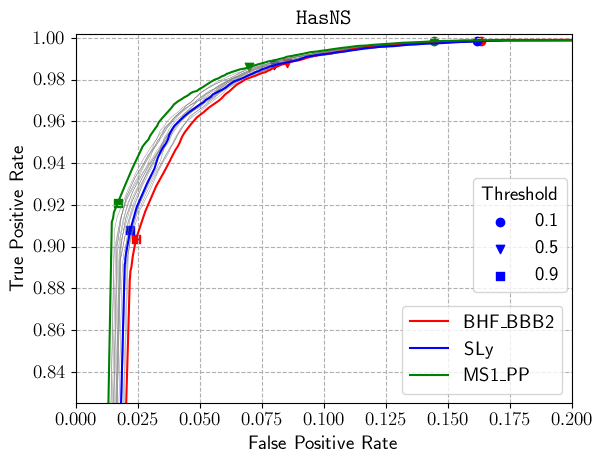
\includegraphics[width=0.45\linewidth]{roc_testing_KNN_NS}
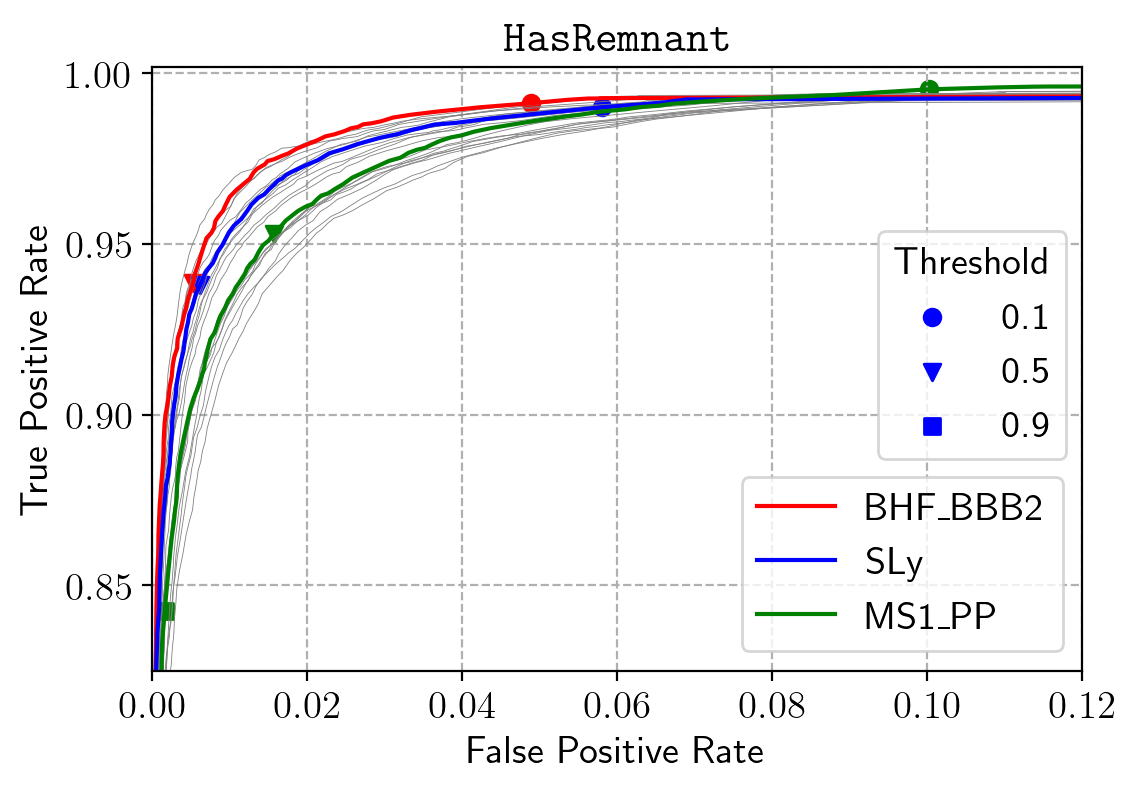
\includegraphics[width=0.45\linewidth]{roc_testing_KNN_REM}
\caption{\ac{ROC} curves for the testing dataset $D_S$ for the \ac{KNN} classifier. The \ac{ROC} of the 23 \ac{EOS} are shown in grey. The \ac{ROC} curves for the \ac{EOS}s with minimum mass ({\tt BHF\_BBB2}), maximum mass ({\tt MS1\_PP}), and {\tt SLy} are highlighted in red, green, and blue, respectively. The circle, triangle, and square markers denote values for score thresholds of 0.1, 0.5, and 0.9, respectively.}
\label{fig:rocO2_KNN}
\end{figure*}

\begin{figure*}[h]
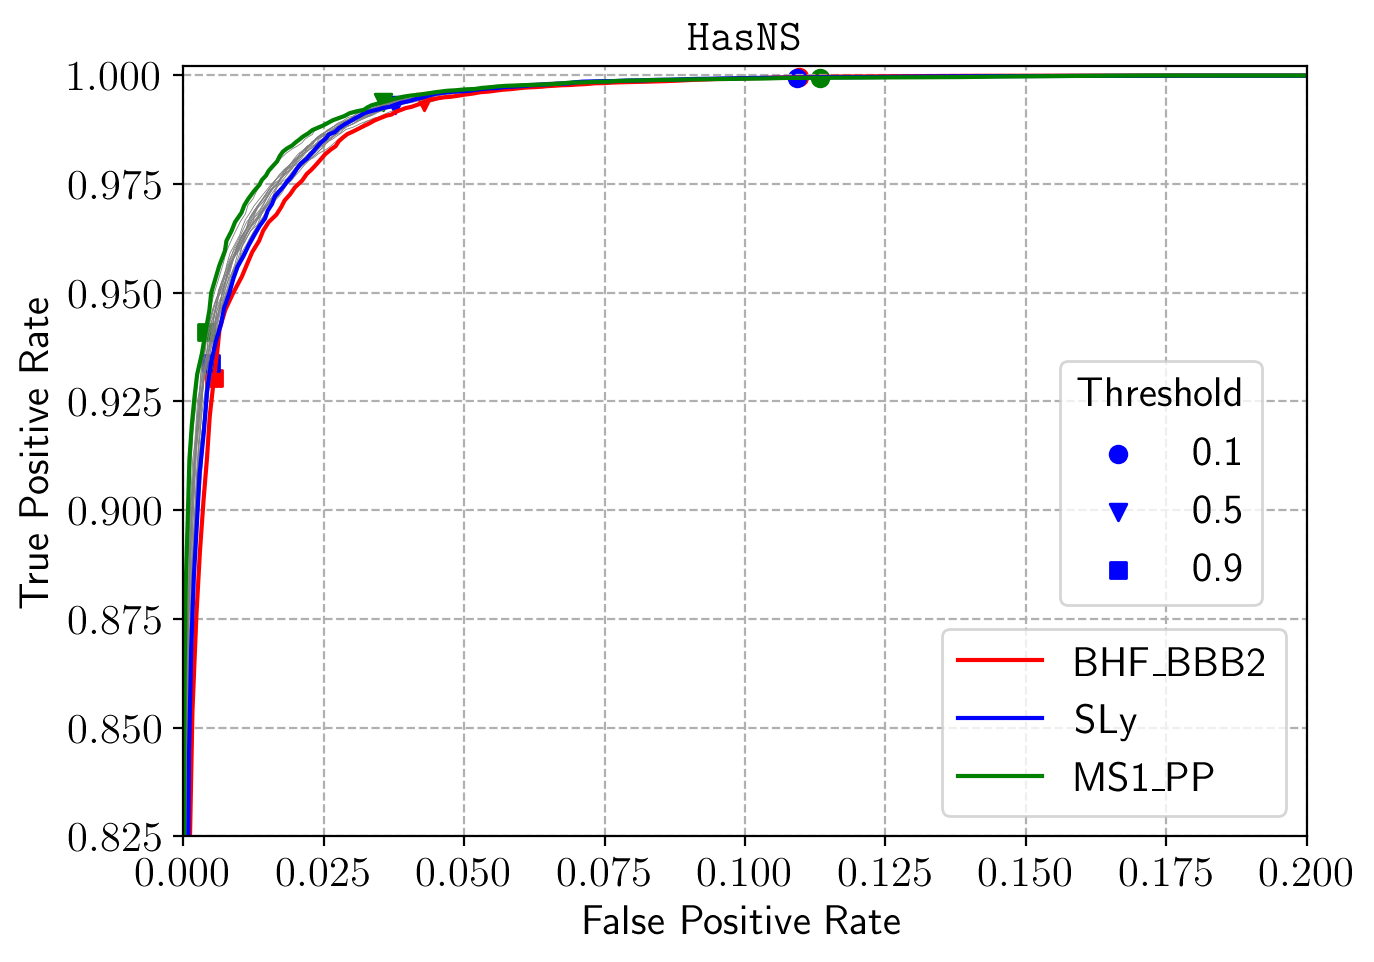
\includegraphics[width=0.45\linewidth]{roc_testing_RF_NS}
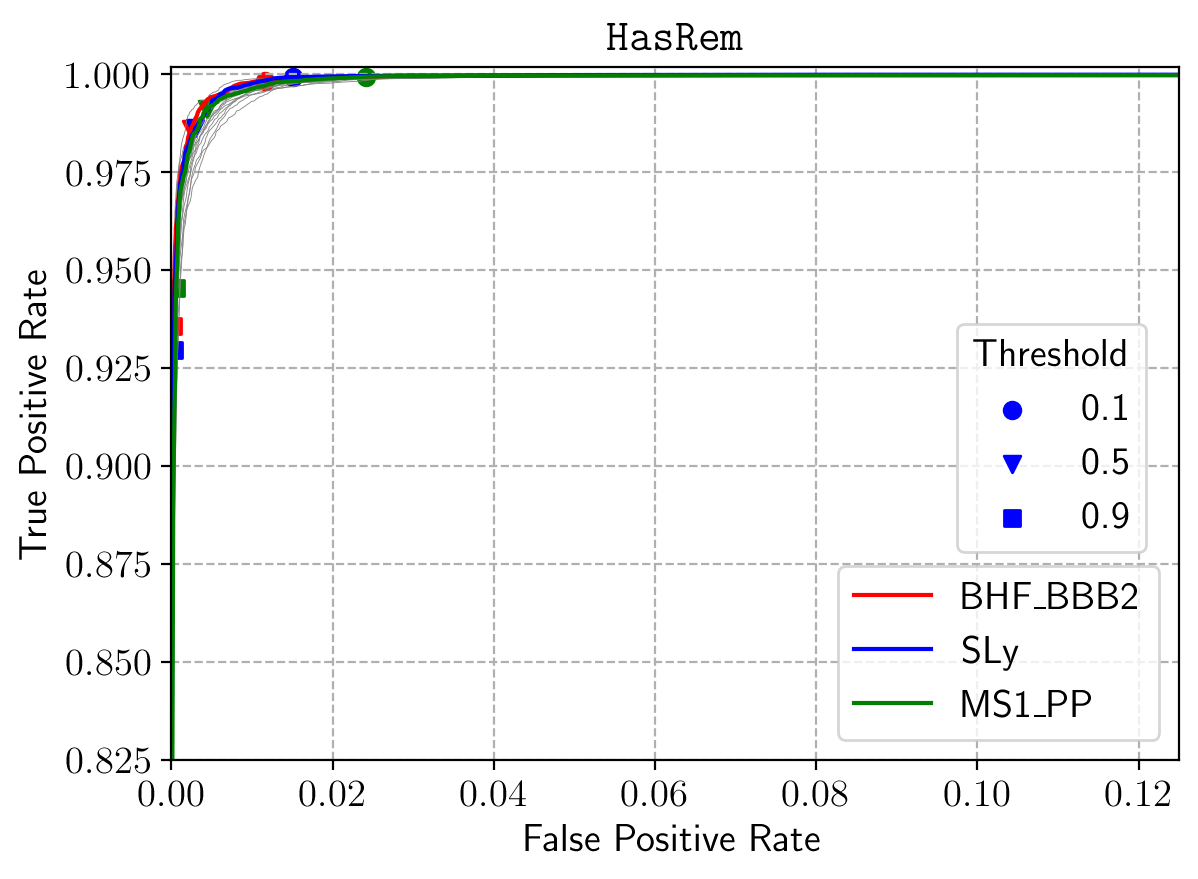
\includegraphics[width=0.45\linewidth]{roc_testing_RF_REM}
\caption{\ac{ROC} curves for the testing dataset $D_S$ for the \ac{RF} classifier. The \ac{ROC} of the 23 \ac{EOS} are shown in grey. The \ac{ROC} curves for the \ac{EOS}s with minimum mass ({\tt BHF\_BBB2}), maximum mass ({\tt MS1\_PP}), and {\tt SLy} are highlighted in red, green, and blue, respectively. The circle, triangle, and square markers denote values for score thresholds of 0.1, 0.5, and 0.9, respectively.}
\label{fig:rocO2_RF}
\end{figure*}

The left and right panels of Fig.~\ref{fig:rocO2_KNN} show the \hasns\ and \hasrem\ \ac{ROC} curves for the \ac{KNN} algorithm, respectively. The analogous curves for the \ac{RF}
classifier are shown in Fig.~\ref{fig:rocO2_RF}. The \ac{ROC} curves for the 23 \ac{EOS} are plotted in grey with three of them highlighted in color: {\tt BHF\_BBB2}, the \ac{EOS} with
lowest maximum mass for the NS \todo{ref needed here}, {\tt MS1\_PP}, the \ac{EOS} with largest maximum mass for the \ac{NS} \todo{ref needed here}, and {\tt SLy}, which allows for a
maximum mass of $2.05 M_\odot$ and is the standard \ac{EOS} used in \ac{LVK} low-latency investigations~\cite{Chaudhary:2023vec} \mmt{[MMT: I got the masses from the em bright git, maybe Sushant knows the references : https://arxiv.org/pdf/2104.08681.pdf Link to Shaon's Paper]}. The markers denote different thresholds for the Bayesian
probabilities $P_M(I|{\bf A})$. 


The two classifiers perform consistently across all \ac{EOS}s. The \ac{TPR} for a score threshold of $0.5$ is around $0.99$ for both \hasns\ and \hasrem. A comparison of the
\hasns\ and \hasrem\ \ac{ROC} curves for each algorithm shows that the \ac{FPR} for \hasns\ is generally higher than the \ac{FPR} for \hasrem\ at a given threshold. Thus the algorithms
typically do a better job in classifying \hasrem\ than \hasns. A separate comparison of the \ac{KNN} and \ac{RF} \ac{ROC} curves for \hasns\ and \hasrem\ shows that both algorithms perform
similarly on the testing dataset, with \ac{RF} giving slightly higher \ac{TPR} and lower \ac{FPR} than \ac{KNN} at a fixed threshold. 

\subsection{Computation of the Bayesian probabilities}

Once the algorithms are trained and tested, we compute the Bayesian
probabilities defined in the Section~\ref{bayesian_probs}, in terms of the 
output of the algorithms (fractions of neighbors and fractions of trees, 
respectively). In order to obtain the probabilities given in 
Equations~\ref{bayes-hasns} and~\ref{bayes-hasrem} one needs to apply
 the algorithm on known events, which are the events from the data set $D$, already used for training and testing the algorithms in the previous subsection. More concretely, we evaluate these probabilities on the testing set $D_S$.

\begin{figure*}%[h]
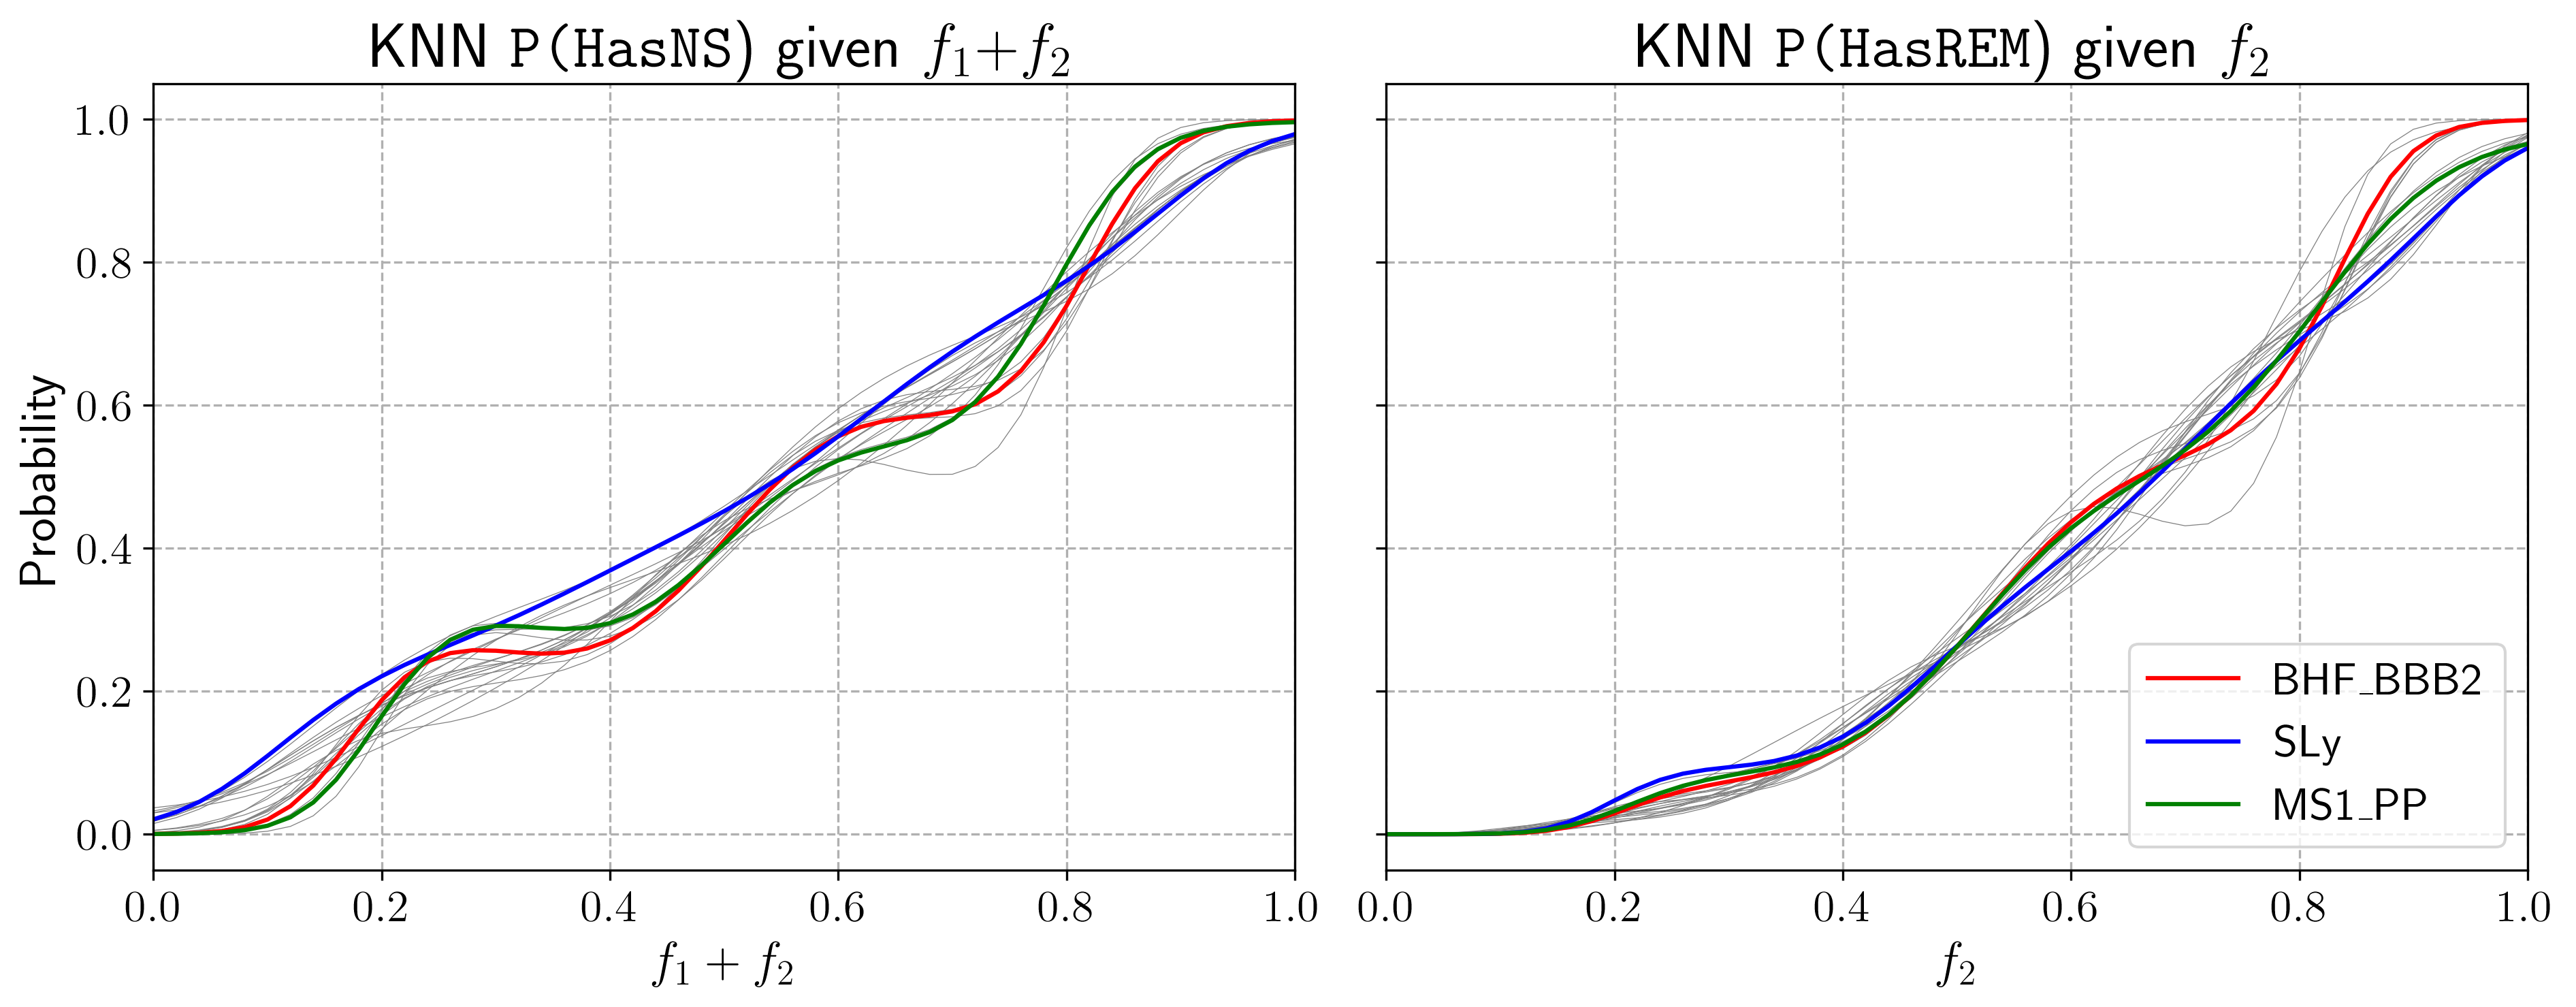
\includegraphics[width=0.65\linewidth]{KNN_3_eos_prob_plots}
\caption{Fits of the Bayesian probabilities as functions of the fraction of neighbors from \ac{KNN}. The left panel corresponds to the probability for \hasns\ and the right panel, to \hasrem\ . The different colors denote the equations of state. Generally, the curves increase with the fraction of neighbors, except of some fluctuations due to having a finite data set.}
\label{fig:bayesian_prob_fits_KNN}
\end{figure*}

\begin{figure*}%[h]
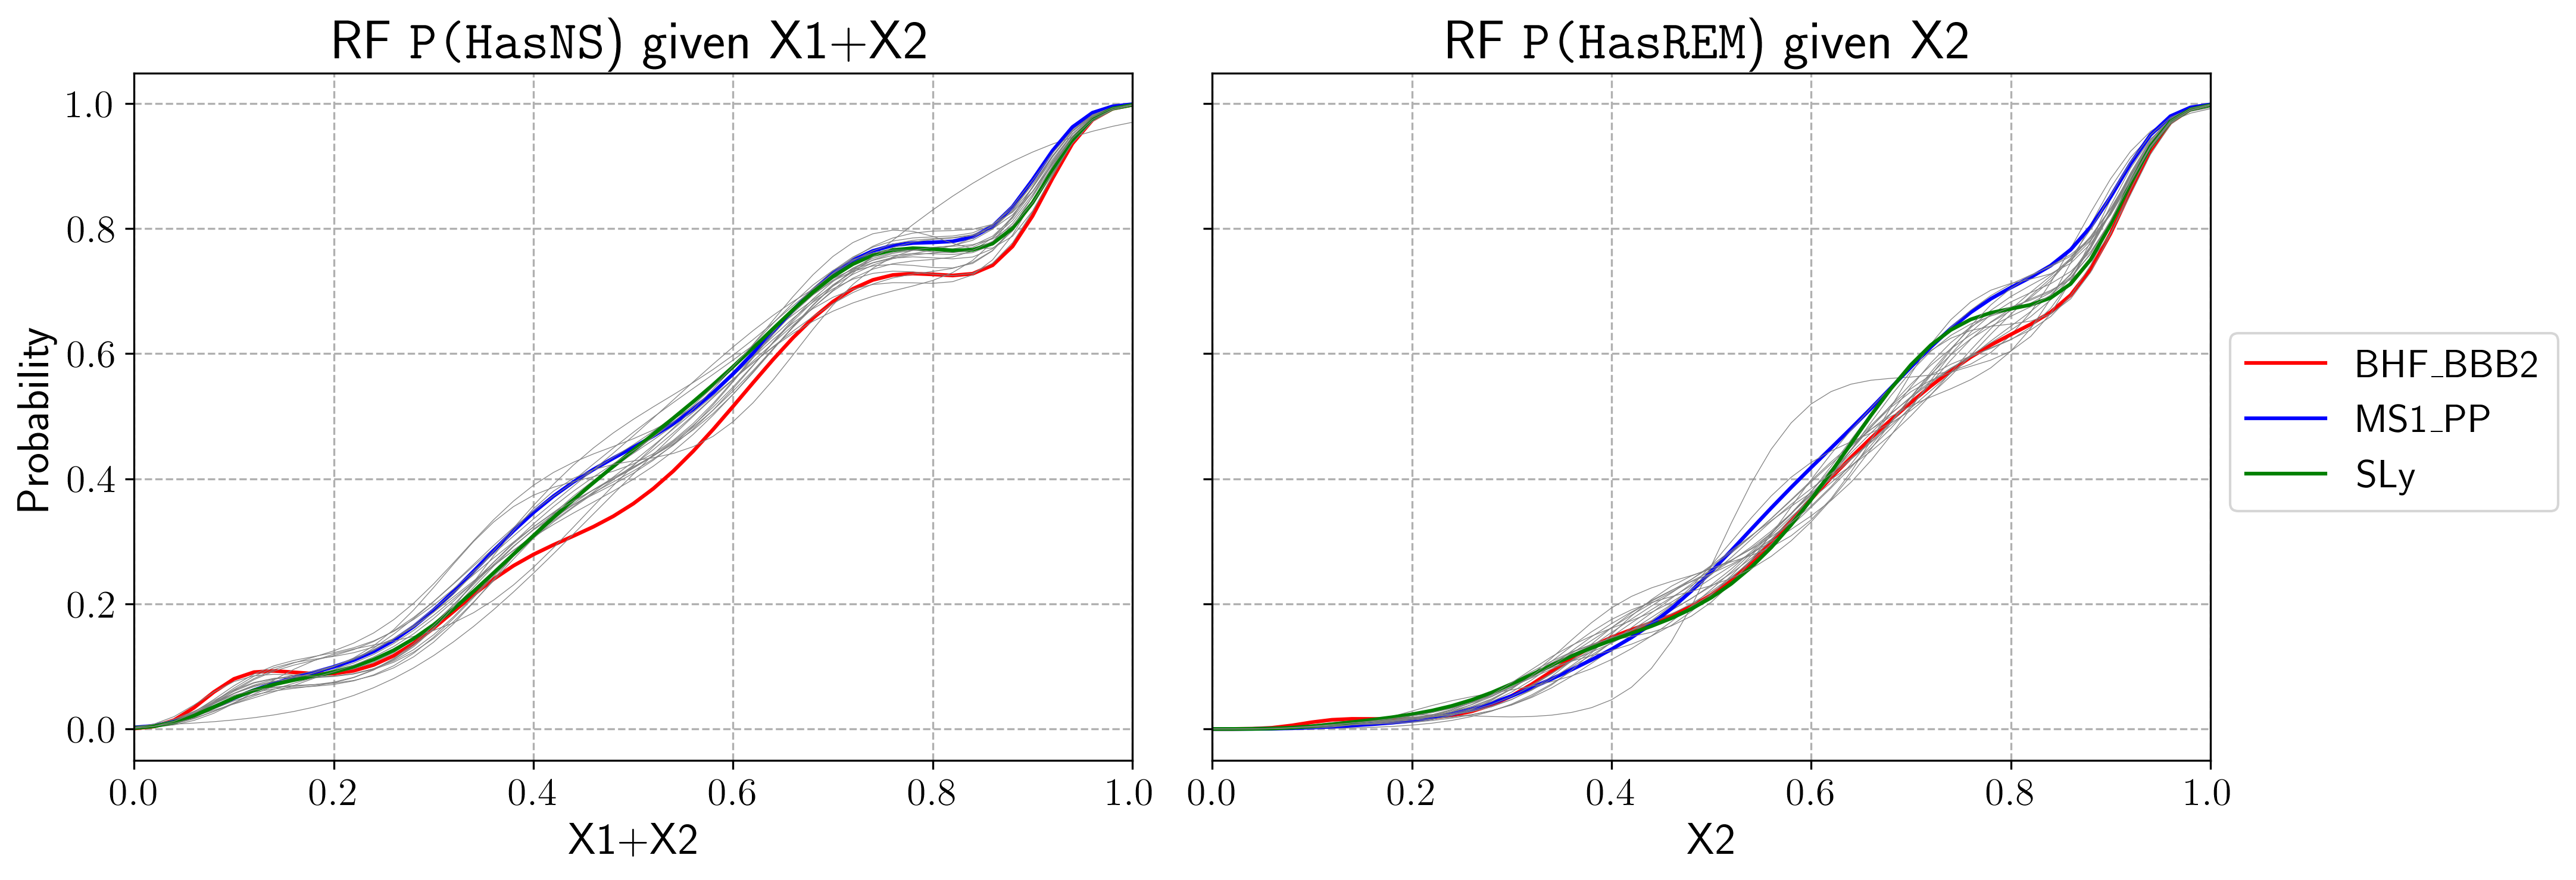
\includegraphics[width=0.65\linewidth]{RF_3_eos_prob_plots}
\caption{Fits of the Bayesian probabilities as functions of the fraction of trees from \ac{RF}. As in Figure~\ref{fig:bayesian_prob_fits_KNN}, the left panel corresponds to the probability for \hasns\ and the right panel, to \hasrem\ . Again, the different colors denote the equations of state. In this case all the fits increase with the fraction of trees.}
\label{fig:bayesian_prob_fits_RF}
\end{figure*}

In Figs.~\ref{fig:bayesian_prob_fits_KNN} and~\ref{fig:bayesian_prob_fits_RF}, 
we show the fits of  the results with a Gaussian Process Regression,
performed as explained in the Section~\ref{bayesian_probs}. In this figures we show
the fits for each EOS, but one can always get a single marginalized probability
applying the Bayes factors. The fitted curves generally increase with the number of neighbors/trees, except of some fluctuations due to the fact that the data set is finite, which results in some noise. The fits also have a
sigmoid-like shape, but that depends on the choice of the EOS. Both \ac{KNN}
and \ac{RF} give fits that have a similar shape. Indeed, both show a slower
increase of $P(\hasrem)$ for a low fraction $f_2$ compared to $P(\hasns)$.
However, \ac{RF} shows a small plateau on the $P(\hasns)$ (and also on
$P(\hasrem)$) for fractions of trees around $0.8$, and that is something that
\ac{KNN} does not reproduce. We highlight the same equations of state as in
Figs.~\ref{fig:rocO2_KNN} and~\ref{fig:rocO2_RF}.

\subsection{Performance on new events}

As stated in the Section~\ref{bayesian_probs}, the fits of the probabilities
$P_J(I|{\bf A}_{\bf X})$ for each EOS ($J=1,\dots 23$) can be tabulated and
used to compute the marginalized probabilities $P_M(\hasns|{\bf A}_{\bf E})$
and $P_M(\hasrem|{\bf A}_{\bf E})$ for any new event $\bf E$ with algorithm
outcome $\bf A_{E}$.  We classify the events from MDC and compute the ROC curves according to the ground truth of
the injected events, which can be seen in Figs.~\ref{fig:rocMDC_KNN}
and~\ref{fig:rocMDC_RF}. We separate the ROC curves for the different pipelines
involved in the dataset (GstLAL,  PyCBC~\cite{Usman:2015kfa},
SPIIR~\cite{Chu:2020pjv} and MBTA~\cite{Adams:2015ulm}). Notice that the curves are very similar even though the algorithms were trained (and also the Bayesian probabilities were fitted) using exclusively GstLAL.

Figure~\ref{fig:rocMDC_KNN} depicts the curves for \ac{KNN}.  In the case of
\hasns\ (left panel), it gives a true positive rate of $\sim 0.975$ for a
threshold of $0.5$ and less than a false positive rate of $0.2$ for all the
pipelines except of SPIIR. Regarding \hasrem\ (right panel), \ac{KNN}. gives a
false positive rate slightly higher than $0.2$ for all the pipelines except of
GstLAL when fixing the threshold to $0.5$, but the true positive rate stays
around $0.975$. In this case, SPIIR behaves similarly to the rest of the pipelines. 

In Fig.~\ref{fig:rocMDC_RF} we showcase the results for \ac{RF}.  The curves
are similar to the ones in Fig.~\ref{fig:rocMDC_KNN}, having a steeper shape for \hasns\ (left panel) and thus giving high true positive rates and low false positive rates at a given threshold. SPIIR also performs poorly for \ac{RF}. When it comes to \hasrem\ (right panel), the false positive rates increase as for \ac{KNN}, and it outperforms on GstLAL compared to the rest of the pipelines.  

One can note that, when applied to a new data set, the algorithms perform better on \hasns\ rather than on \hasrem\, as opposed to what happenned with the testing data set $D_S$ from O2 (see Figs.~\ref{fig:rocO2_KNN} and~\ref{fig:rocO2_RF}). Moreover, \ac{KNN} outperforms \ac{RF} when it comes to \hasrem\ (especially on other pipelines than GstLAL), and both algorithms work better for events injected on GstLAL, which is the pipeline exclusively used in the training data set. Due to the hard cuts applied by \ac{RF} and the fact that it has been trained only with GstLAL injections, this algorithm is less adaptable than \ac{KNN}, and that is why the ROC curves are not as steep as for \ac{KNN} when classifying data from other pipelines. 

%\begin{comment}
%performs very well for \hasns achieving a true positive rate very close to
%unity with a very small false positive rate. We observe that SPIIR pipeline
%deviates from the good behaviour. For \hasrem the overall performance is
%slightly worse, getting higher false positive rate, but in turn all
%pipelines behave equally good. In Fig.~\ref{fig:rocMDC_RF} we showcase the results for \ac{RF}. As with \ac{KNN} the results are very good, with steep ROC curves. For \hasns spiir pipeline deviates less from the rest, getting higher positive rates for the same false positives than with \ac{KNN}. In the case of \hasrem the curves of the different pipelines behave a bit more differently from each other.
%\end{comment}

\begin{figure*}%[h]
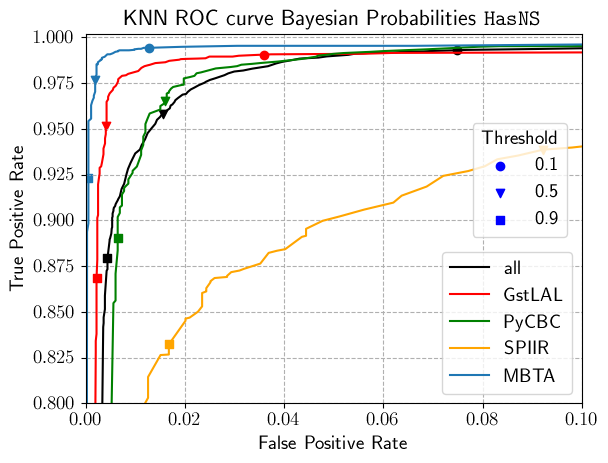
\includegraphics[width=0.45\linewidth]{roc_mdc_KNN_NS}
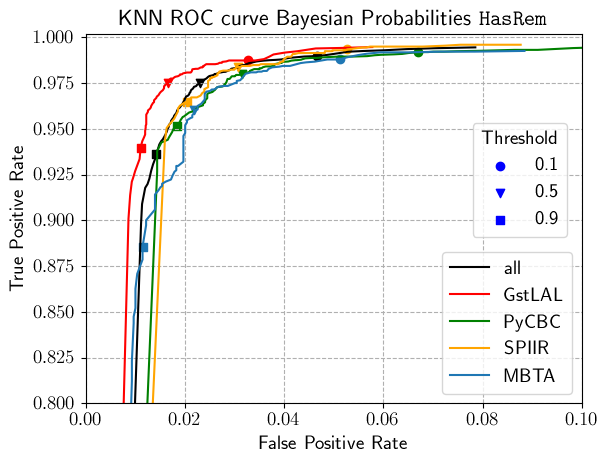
\includegraphics[width=0.45\linewidth]{roc_mdc_KNN_REM}
\caption{ROC curves of Bayesian probability marginalized
    for the 23 EoSs for MDC11 dataset using \ac{KNN} classifier.}
\label{fig:rocMDC_KNN}
\end{figure*}

\begin{figure*}%[h]
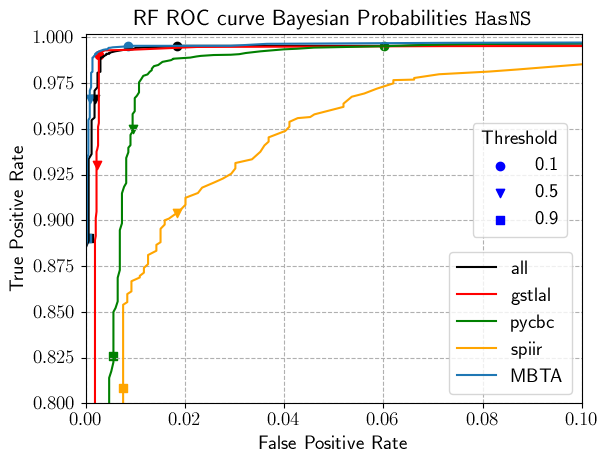
\includegraphics[width=0.45\linewidth]{roc_mdc_RF_NS}
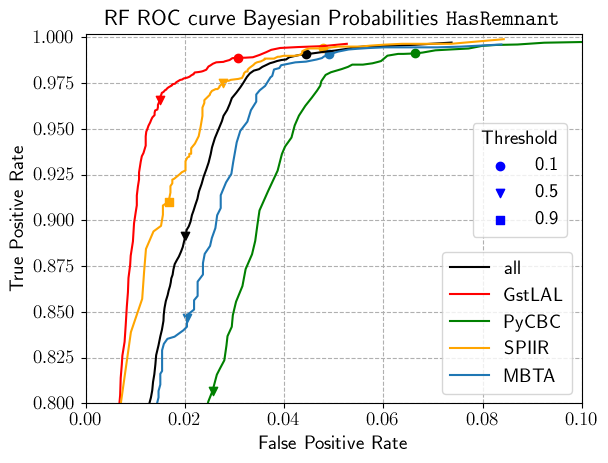
\includegraphics[width=0.45\linewidth]{roc_mdc_RF_REM}
\caption{ROC curves of Bayesian probability marginalized for the 23 EoSs for MDC11 dataset using \ac{RF} classifier.}
\label{fig:rocMDC_RF}
\end{figure*}

We also applied the tabulated Bayesian probabilities to classify real events
from the O3 LVK run~\cite{LIGOScientific:2020ibl, LIGOScientific:2021djp}.  In Table~\ref{tab:real_data_bayesian} we depict some of the most significant events of the LVK third observing run, labeling them with their event ID and the GraceDB\footnote{\href{https://gracedb.ligo.org/}https://gracedb.ligo.org/} ID.  We show the marginalized Bayesian probabilities for both \hasns\ and \hasrem\ computed with 
\ac{RF} and \ac{KNN}. For the first two events (GW170817 and GW190425),
$P_M(\hasns)$ and $P_M(\hasrem)$ are very close to 1, meaning that these events
correspond to BNS mergers, as shown in~\cite{LIGOScientific:2020ibl,LIGOScientific:2021djp}. 
For GW190426 and GW200115, $P_M(\hasns) \sim 1$, but
$P_M(\hasrem) = 0$, which correspond to NSBH mergers, and agree 
with~\cite{LIGOScientific:2020ibl, LIGOScientific:2021djp}. Finally, GW190814 and GW190924,
have non-zero $P_M(\hasns)$ (indeed, \ac{KNN} gives a probability higher than
0.5 for GW190814). The results in~\cite{LIGOScientific:2020ibl, LIGOScientific:2021djp} show that these events are high mass-ratio BBH mergers. The fact that the component masses are very different from each other (and the lower mass is close to the NS limit) might have led to these non-zero probabilities. Moreover, for GW190814 \ac{KNN} gives a probability higher than 0.5 for \hasns, which differs considerably from what \ac{RF} predicts, which is only a 0.042. This is because for this event, regarding at the posterior of the secondary mass, only three out of twenty three equations of state are compatible with a NS. Since \ac{RF} applies a hard cut on the EOS, $P_M(\hasns|{\bf A}_{\bf E})$ will be low. However, \ac{KNN} depends on the neighbors surrounding the event, and the mass gap is not filled enough in the training dataset, which makes that the closer neighbors are NSs. 

\begin{table}[]
\begin{tabular}{c|cc|cc}
\hline
\multicolumn{1}{c|}{}      & \multicolumn{2}{c|}{$P_M(\hasns|{\bf A}_{\bf E})$}                                                & \multicolumn{2}{c}{$P_M(\hasrem|{\bf A}_{\bf E})$}                                                \\ \hline
\multicolumn{1}{c|}{event ID}   & \multicolumn{1}{c}{RF} & \multicolumn{1}{c}{KNN}  & \multicolumn{1}{c}{RF} & \multicolumn{1}{c}{KNN} \\ \hline
GW170817                                   & 0.998                   & 0.989                    & 0.997                   & 0.985                                  \\
GW190425                                   & 0.998                   & 0.989                    & 0.997                   & 0.985                            \\
GW190426                                   & 0.997                   & 0.985                    & 0.000                   & 0.000                     \\
GW190814                                   & 0.042                   & 0.567                   & 0.000                  & 0.000                      \\
GW190924                                   & 0.012                   & 0.054                   & 0.000               & 0.000                       \\               
GW200115                                   & 0.998                   & 0.989                   & 0.000                  & 0.000                           \\
\hline
\end{tabular}
\caption{Bayesian probabilities of some real GW events from the O3 observing run. GW170817 and GW190425 actually correspond to BNS mergers; GW190426 and GW200115 are NSBH mergers, and GW190814 and GW190924 are BBH mergers. The reason why $P_M(\hasns|{\bf A}_{\bf E})$ is not zero for GW190814 and GW190924 is because the inferred secondary mass is located close to the threshold value of the mass of a NS. The probabilities are truncated to $10^{-3}$, which means that there is not a zero Bayesian probability, but it is actually smaller than $10^{-3}$.}
\label{tab:real_data_bayesian}
\end{table}

In Figs.~\ref{fig:param_sweep_KNN} and~\ref{fig:param_sweep_RF} we depict parameter sweeps that are built using the Bayesian probabilities computed with \ac{KNN} and \ac{RF}, respectively.  These figures show the Bayesian probability for \hasns\ (left column) and for \hasrem\ (right column) for given component masses of the binary system, being $m_1$ the larger mass. The  columns stand for different fixed values of the component spins. The SNR is fixed to 10. One can see that both algorithms perform in a similar way. Regarding $P_M(\hasns)$,  there are no notable differences between the choice of spin values.  There is a small difference between the algorithms: for the third column ($\chi_1 = 0.0$ and $\chi_2$), $P_M(\hasns)$ is larger for bigger $m_1$ in the case of \ac{KNN}. For $P_M(\hasrem)$, both algorithms give almost the same results. The sweeps show that, for a large $\chi_1$, the probability of having a remnant increases for bigger values of the first component mass, $m_1$. As expected, the region in which $P_M(\hasrem) \sim 1$ is inside the region in which $P_M(\hasns) \sim 1$.

Moreover, the parameter sweeps of $P_M(\hasns)$ (left column) for \ac{KNN} seem to be noisier for large primary masses. This is because the algorithm just looks at the closest neighbors, and it only needs few neighbors that are labelled differently to provide a higher probability in a certain region. On the other hand, \ac{RF} applies a hard cut on large primary masses, resulting in a more uniform probability in that region. 

\begin{figure*}%[h]
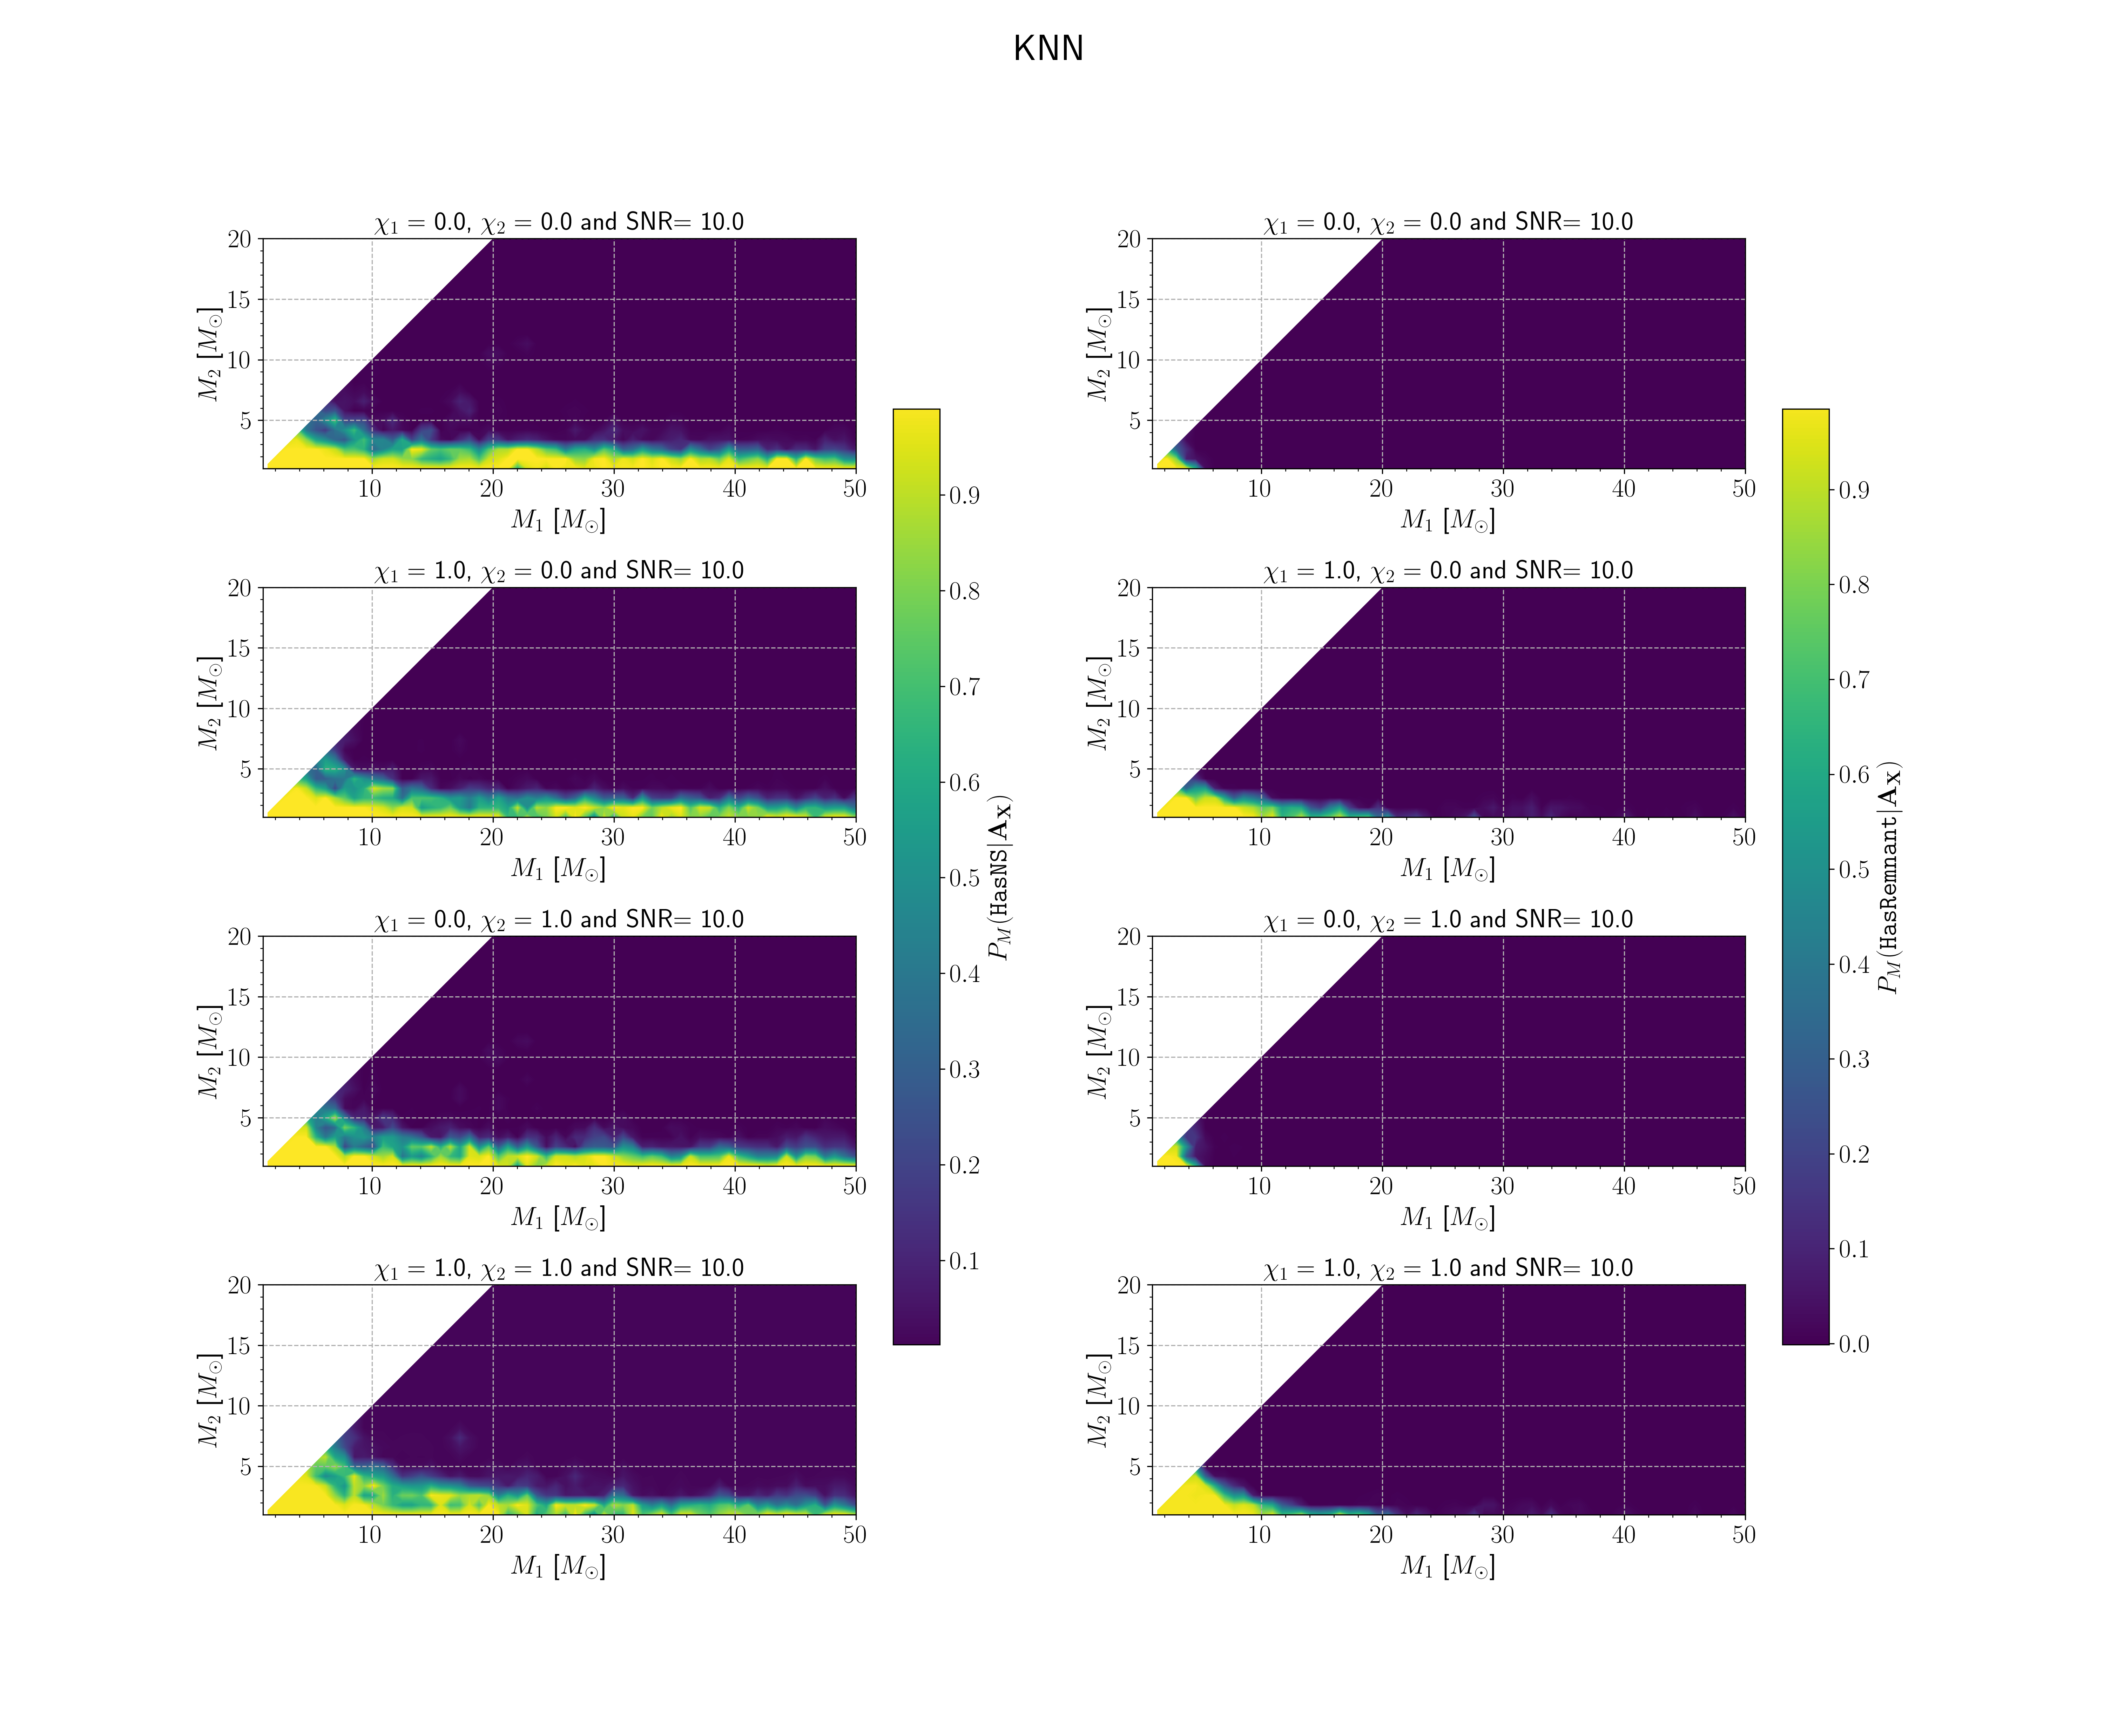
\includegraphics[width=0.7\linewidth]{KNN_parameter_sweep}
    \caption{Parameter sweep obtained with \ac{KNN}. The Bayesian probabilities are shown as a function of the component masses of the binary, where $m_1$ (the bigger mass) is in the horizontal axes and $m_2$, in the vertical. The left panels show $P_M(\hasns)$ and the right panels, $P_M(\hasrem)$. We choose different values of the spin components to evaluate the probability, and they appear in the different rows of the figure.   The SNR is fixed to 10. }
\label{fig:param_sweep_KNN}
\end{figure*}

\begin{figure*}%[h]
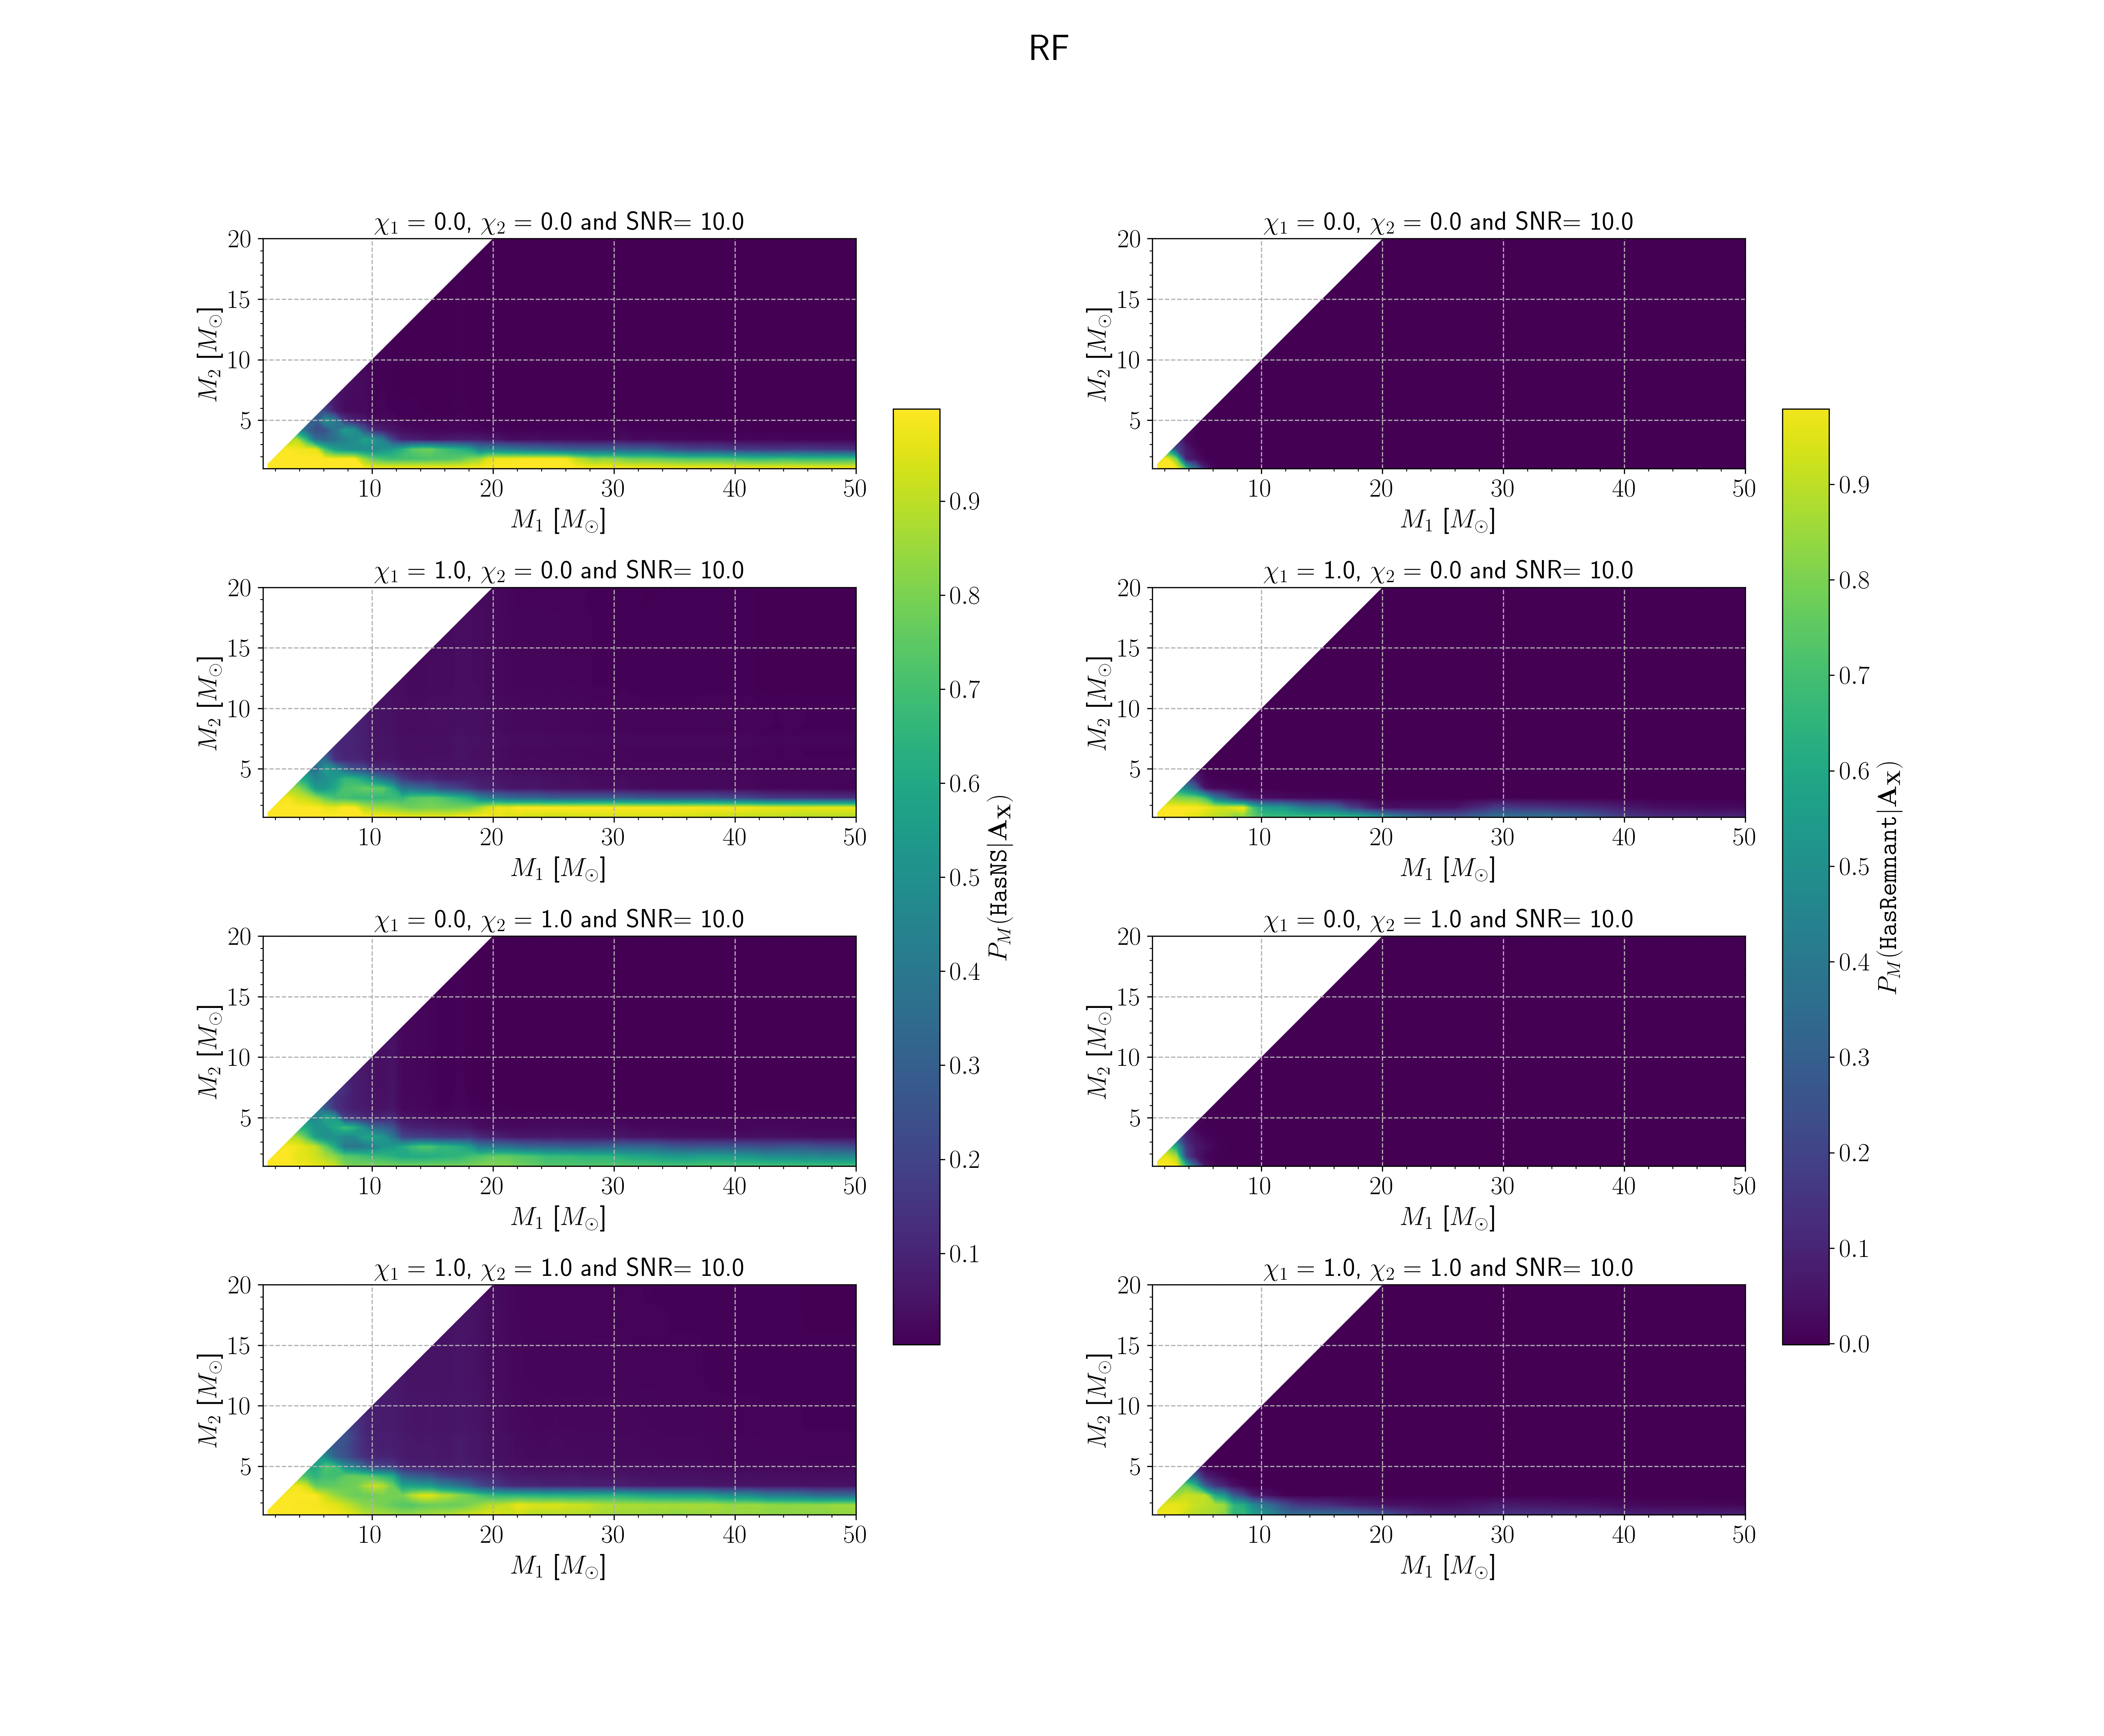
\includegraphics[width=0.7\linewidth]{RF_parameter_sweep}
 \caption{Same as Figure~\ref{fig:param_sweep_KNN}, but now for \ac{RF}.}
\label{fig:param_sweep_RF}
\end{figure*}


%Here are the results for the methods:

%\subsection{KNN Results}

%\mmt{We are only using 5 features, the independent variables: 
%\begin{equation*}
	%\big[m_1,m_2,\chi_1,\chi_2, \rm{SNR}\big]\,.
%\end{equation*}}

\subsubsection{\mmt{Has NS}}
\mmt{The metric we use to compute the distance between neighbors is the \textit{Manhattan} metric (or the Minkowski's $L1$ distance),  which is the distance between two points measured along axes at right angles. Having $p_1(x_1,y_1)$ and $p_2(x_2,y_2)$ the distance will be}
\begin{equation}
	d = |x_1-x_2|+|y_1-y_2|\,.
\end{equation}

\mmt{Moreover, the points are weighted uniformly.  After applying cross-validation,  we get that the optimal number of neighbors is $K_{\rm NS} = 10$, with a mean score $\rm{s_m} = 0:9718355224352762$ and a testing score  $\rm{s_t} = 0.9723828730478842$.} 

%\begin{figure}
%    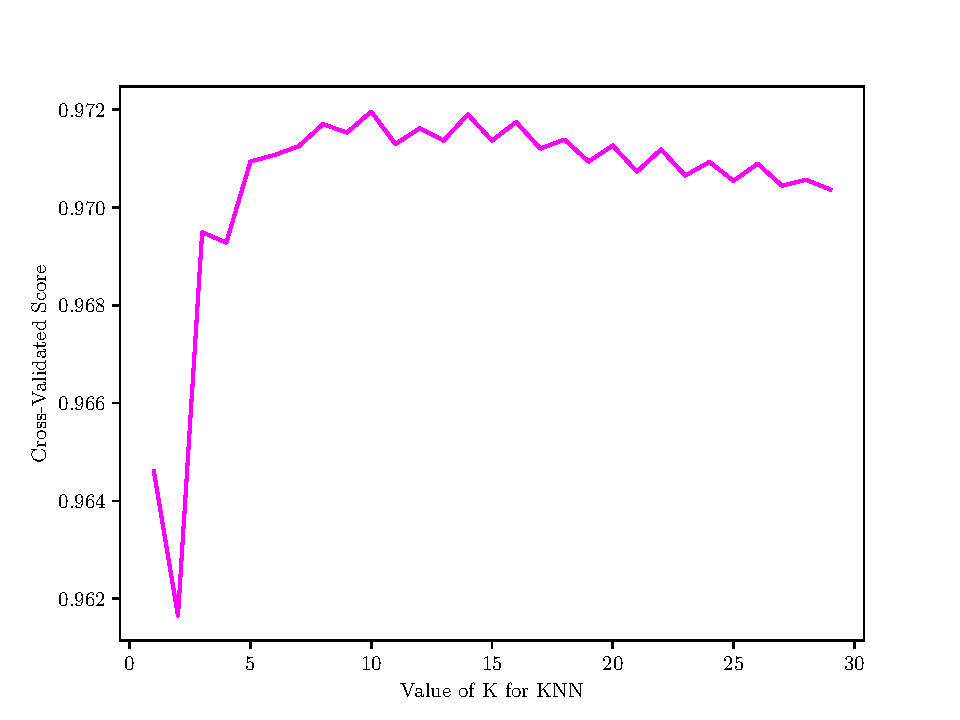
\includegraphics[width = 0.4\textwidth]{CrossValK.pdf}
%    \caption{Score of our KNN model as a function of the number of neighbors. We are considering \textit{HasNS}.}
%    \label{fig:crossvalK}
%\end{figure}
    
\begin{figure}
    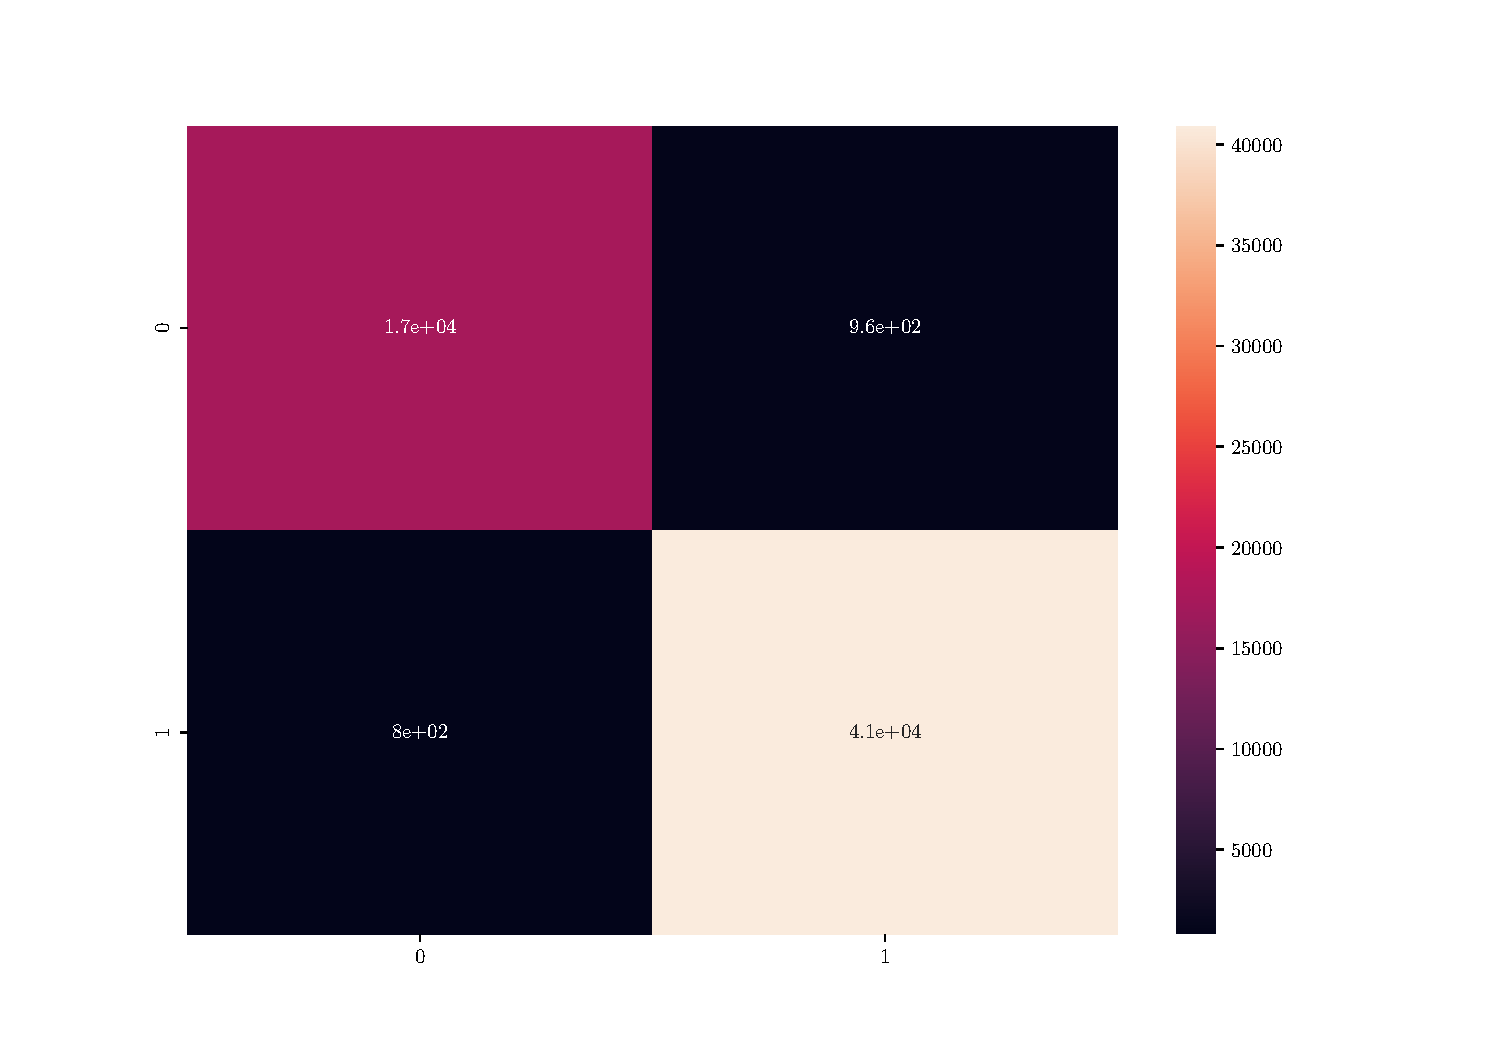
\includegraphics[width=0.45\textwidth]{figs/conf_matrix_NS.pdf}
    \caption{Confusion matrix for our model for \textit{HasNS}, using the independent recovered values. }
    \label{fig:confmat}
\end{figure}

\begin{figure}
    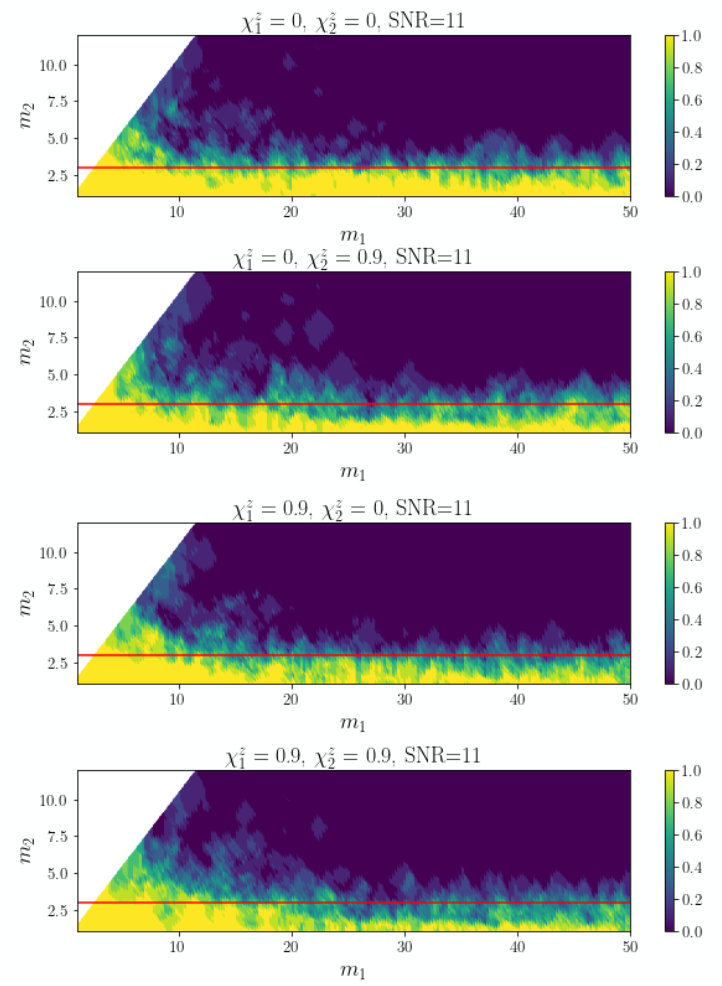
\includegraphics[width = 0.4\textwidth]{plot_fig4_chatt_spins.png}
  %   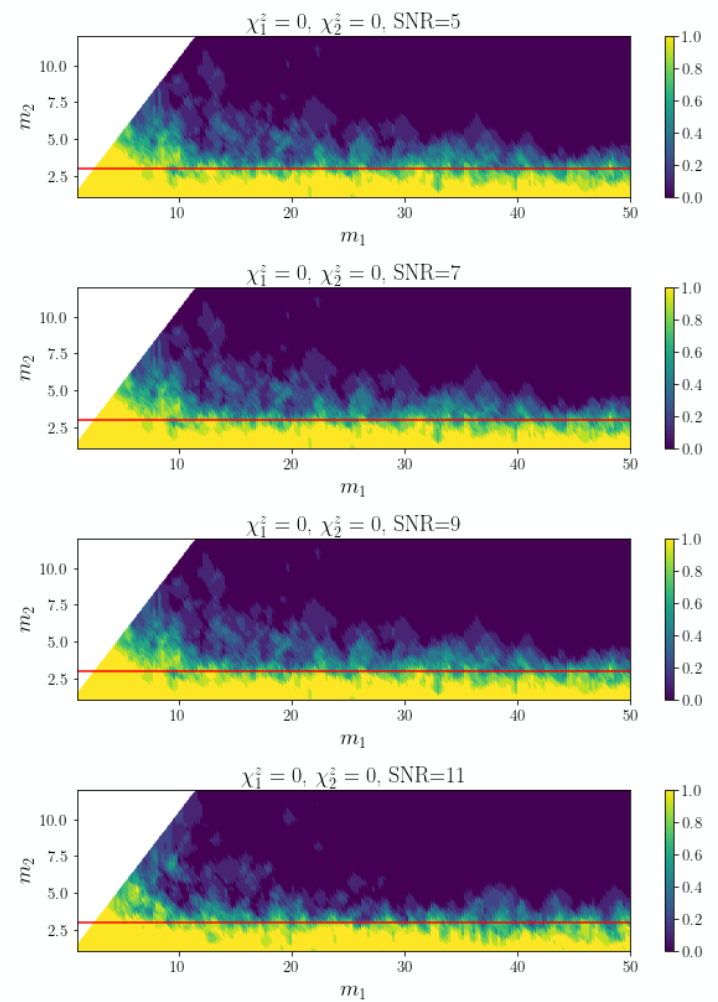
\includegraphics[width = 0.4\textwidth]{/Users/miquelmiravet/Projects/IPAM_LA/ML_group/IPAM2021_ML/algo/classy_KNN/PLOTS_KNN/NS_set/plots_miq/plot_fig4_chatt_snr.png}
    \caption{Probability of having a remnant as a function of the values of the masses. The different panels show the results for different spins. The solid red line depicts the threshold mass for $m_2$.}
    \label{fig:m1m2}
\end{figure}

\begin{figure}
	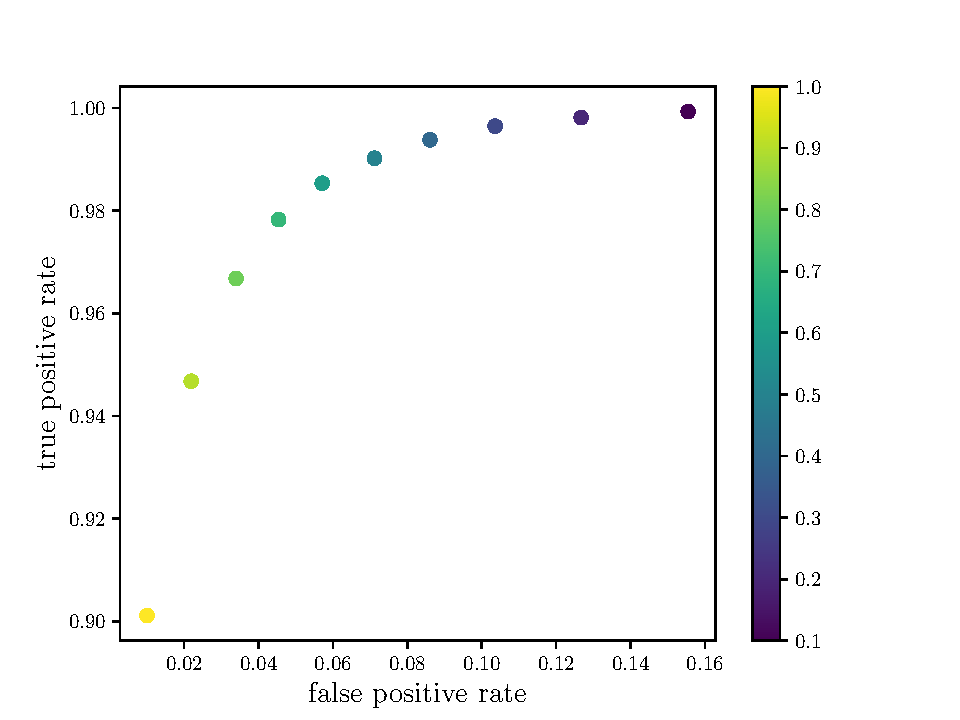
\includegraphics[width =0.4\textwidth]{ROCplot.pdf}
    \caption{Relation of the true and false positive rates as a function of the threshold applied to make the decision between having or not having a remnant. }
    \label{fig:roc}
\end{figure}

\mmt{In Fig.~\ref{fig:crossvalK} you can find how the mean score changes with the number of neighbors of the algorithm.  The confusion matrix appears in Fig.~\ref{fig:confmat}, the probability as a function of $m_1$ and $m_2$  is shown in Figs.~\ref{fig:m1m2}, and the true and false positive rates in terms of the threshold probability appear in Fig.~\ref{fig:roc}.}


 %plots and comments
%\subsection{RF Results}

We apply crossvalidation in the number of trees and depth of the forests for the 23 EoS, fixing the information gain criteria to \texttt{entropy}. We also save the second best option for comparison, and save both forests for each EoS in order to compare the file size. As the goal is to provide a model that can run in a low latency pipeline the amount of memory it can take is limited, even more when there will be 23 different model for the EoS generalization.

In table \ref{tab:RFcross} we present a summary of best and second best hyperparameters found in the crossvalidation for each EoS, along the memory the model occupies and the difference in the score. As we can see, usually a forest with many trees has a second best option with far less that is lighter in memory and achieves a similar performance. The optimum maximum depth is always 15. Also the score achieved for every EoS is similar, and so we check that our accuracy is not NS model dependent.

\begin{table*}[h]
\centering
\begin{tabular}{@{}lcccccccc@{}}
\toprule
                                & \multicolumn{4}{c}{Best}                                & \multicolumn{4}{c}{Second best}                            \\ \midrule
\multicolumn{1}{|l|}{EOS}       & Trees & Depth & Size(MB)    & \multicolumn{1}{c|}{Score}      & Trees & Depth & Size(MB)    & \multicolumn{1}{c|}{$\Delta$score} \\ \midrule
\multicolumn{1}{|l|}{APR4\_BB}  & 300   & 15    & 94.7  & \multicolumn{1}{c|}{0.9683018}  & 50    & 15    & 15.7  & \multicolumn{1}{c|}{3.35e-5}       \\ \midrule
\multicolumn{1}{|l|}{BHF\_BBB2} & 80    & 15    & 24.4  & \multicolumn{1}{c|}{0.9685127}  & 300   & 15    & 91.6  & \multicolumn{1}{c|}{5.16e-5}       \\ \midrule
\multicolumn{1}{|l|}{H4}        & 80    & 15    & 29.6  & \multicolumn{1}{c|}{0.9618587}  & 300   & 15    & 111.4 & \multicolumn{1}{c|}{1.19e-4}       \\ \midrule
\multicolumn{1}{|l|}{HQC18}     & 300   & 15    & 93.7  & \multicolumn{1}{c|}{0.9673755}  & 100   & 15    & 31.3  & \multicolumn{1}{c|}{3.06e-4}       \\ \midrule
\multicolumn{1}{|l|}{KDE0V}     & 300   & 15    & 92.0  & \multicolumn{1}{c|}{0.9673295}  & 80    & 15    & 24.5  & \multicolumn{1}{c|}{2.06e-4}       \\ \midrule
\multicolumn{1}{|l|}{KDE0V1}    & 100   & 15    & 30.9  & \multicolumn{1}{c|}{0.96704954} & 80    & 15    & 24.5  & \multicolumn{1}{c|}{3.43e-5}       \\ \midrule
\multicolumn{1}{|l|}{MPA1}      & 80    & 15    & 27.2  & \multicolumn{1}{c|}{0.96601225} & 300   & 15    & 102.1 & \multicolumn{1}{c|}{8.19e-5}       \\ \midrule
\multicolumn{1}{|l|}{MS1\_PP}   & 300   & 15    & 113.5 & \multicolumn{1}{c|}{0.96563534} & 80    & 15    & 30.2  & \multicolumn{1}{c|}{1.15e-4}       \\ \midrule
\multicolumn{1}{|l|}{MS1B\_PP}  & 300   & 15    & 114.2 & \multicolumn{1}{c|}{0.96555340} & 100   & 15    & 38.0  & \multicolumn{1}{c|}{1.97e-4}       \\ \midrule
\multicolumn{1}{|l|}{RS}        & 300   & 15    & 103.8 & \multicolumn{1}{c|}{0.96447350} & 80    & 15    & 27.6  & \multicolumn{1}{c|}{2.36e-4}       \\ \midrule
\multicolumn{1}{|l|}{SK255}     & 300   & 15    & 105.8 & \multicolumn{1}{c|}{0.96472405} & 100   & 15    & 35.5  & \multicolumn{1}{c|}{3.69e-4}       \\ \midrule
\multicolumn{1}{|l|}{SK272}     & 300   & 15    & 109.0 & \multicolumn{1}{c|}{0.96401816} & 100   & 15    & 36.4  & \multicolumn{1}{c|}{1.99e-4}       \\ \midrule
\multicolumn{1}{|l|}{SKI2}      & 50    & 15    & 18.8  & \multicolumn{1}{c|}{0.96242338} & 300   & 15    & 112.8 & \multicolumn{1}{c|}{8.37e-5}       \\ \midrule
\multicolumn{1}{|l|}{SKI3}      & 50    & 15    & 19.0  & \multicolumn{1}{c|}{0.96174537} & 100   & 15    & 38.1  & \multicolumn{1}{c|}{6.62e-5}       \\ \midrule
\multicolumn{1}{|l|}{SKI4}      & 300   & 15    & 100.6 & \multicolumn{1}{c|}{0.96598969} & 30    & 15    & 9.8   & \multicolumn{1}{c|}{8.37e-5}       \\ \midrule
\multicolumn{1}{|l|}{SKI5}      & 100   & 15    & 38.2  & \multicolumn{1}{c|}{0.96343381} & 80    & 15    & 30.4  & \multicolumn{1}{c|}{1.16e-4}       \\ \midrule
\multicolumn{1}{|l|}{SKI6}      & 300   & 15    & 101.7 & \multicolumn{1}{c|}{0.96586928} & 30    & 15    & 10.0  & \multicolumn{1}{c|}{2.17e-4}       \\ \midrule
\multicolumn{1}{|l|}{SKMP}      & 300   & 15    & 100.2 & \multicolumn{1}{c|}{0.96544567} & 80    & 15    & 26.9  & \multicolumn{1}{c|}{1.69e-4}       \\ \midrule
\multicolumn{1}{|l|}{SKOP}      & 100   & 15    & 32.3  & \multicolumn{1}{c|}{0.96610459} & 300   & 15    & 96.2  & \multicolumn{1}{c|}{6.85e-5}       \\ \midrule
\multicolumn{1}{|l|}{SLy}       & 80    & 15    & 25.3  & \multicolumn{1}{c|}{0.96728884} & 300   & 15    & 95.2  & \multicolumn{1}{c|}{8.49e-5}       \\ \midrule
\multicolumn{1}{|l|}{SLY2}      & 100   & 15    & 31.8  & \multicolumn{1}{c|}{0.96745868} & 80    & 15    & 25.4  & \multicolumn{1}{c|}{2.38e-4}       \\ \midrule
\multicolumn{1}{|l|}{SLY9}      & 300   & 15    & 101.6 & \multicolumn{1}{c|}{0.96605993} & 100   & 15    & 34.1  & \multicolumn{1}{c|}{1.51e-4}       \\ \midrule
SLY230A                         & 300   & 15    & 95.5  & 0.96714915                      & 100   & 15    & 31.9  & 2.53e-4                            \\ \bottomrule
\end{tabular}
\caption{Comparison of the best and second best RF models obtained during crossvalidation for all EoS. We show the file size in MB of the forest, and the difference in score between the two options.}
\label{tab:RFcross}
\end{table*}

To simplify the model and according to the results of crossvalidation, we train the final forests for all EoS with 50 trees and 15 maximum depth. In figure \ref{fig:RF_roc} we show the ROC curves for all models to give an idea of the performance. Notice that HasREM performs better than HasNS. The ourperformance of HasREM against HasNS in RF is even more noticeable in the histograms in figures \ref{fig:RF_hist_BHFBBB2}, \ref{fig:RF_hist_SLY} and \ref{fig:RF_hist_MS1PP} for the highlighted EoS, where the bars of asigned probabilities do not intersect each other and therefore there exists a threshold value for perfect classification in the testing dataset.

\begin{figure}
\centering
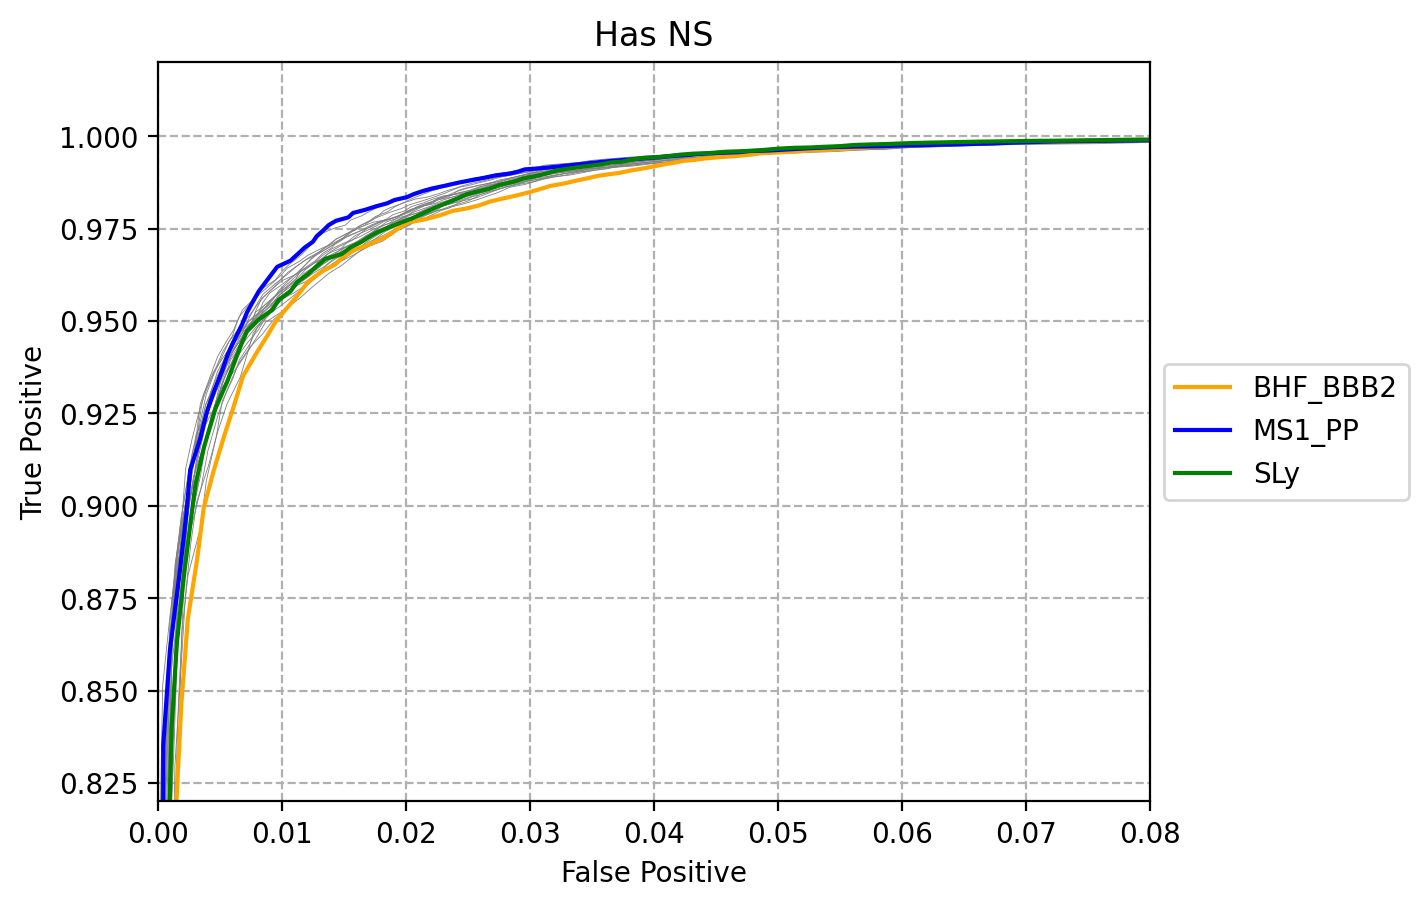
\includegraphics[width=0.45\textwidth]{/figs/HasNS_roc}
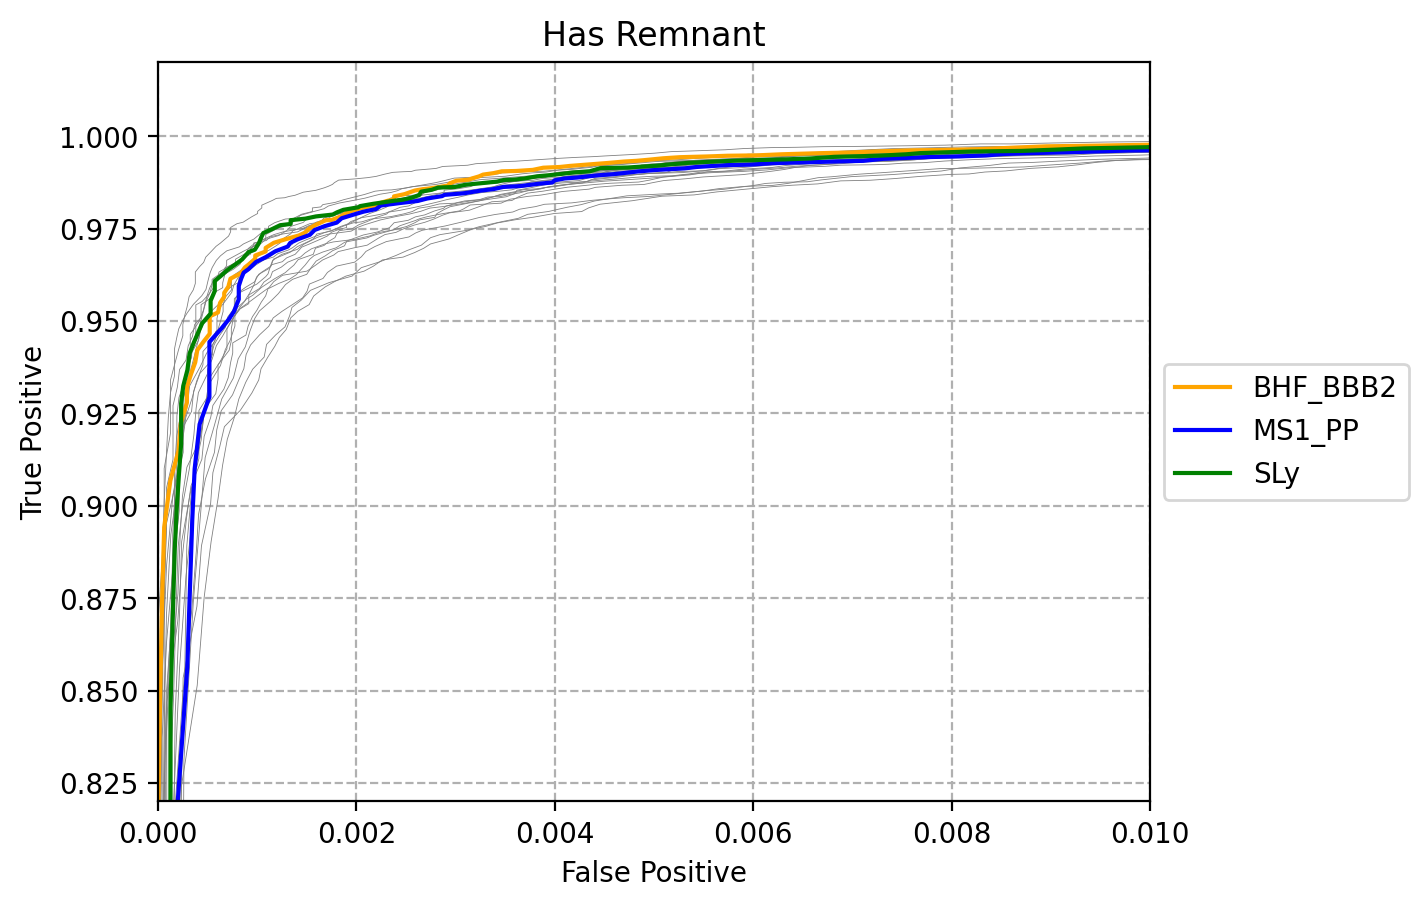
\includegraphics[width=0.45\textwidth]{/figs/HasREM_roc}
\caption{\label{fig:RF_roc} ROC curves}
\end{figure}

\begin{figure}
\centering
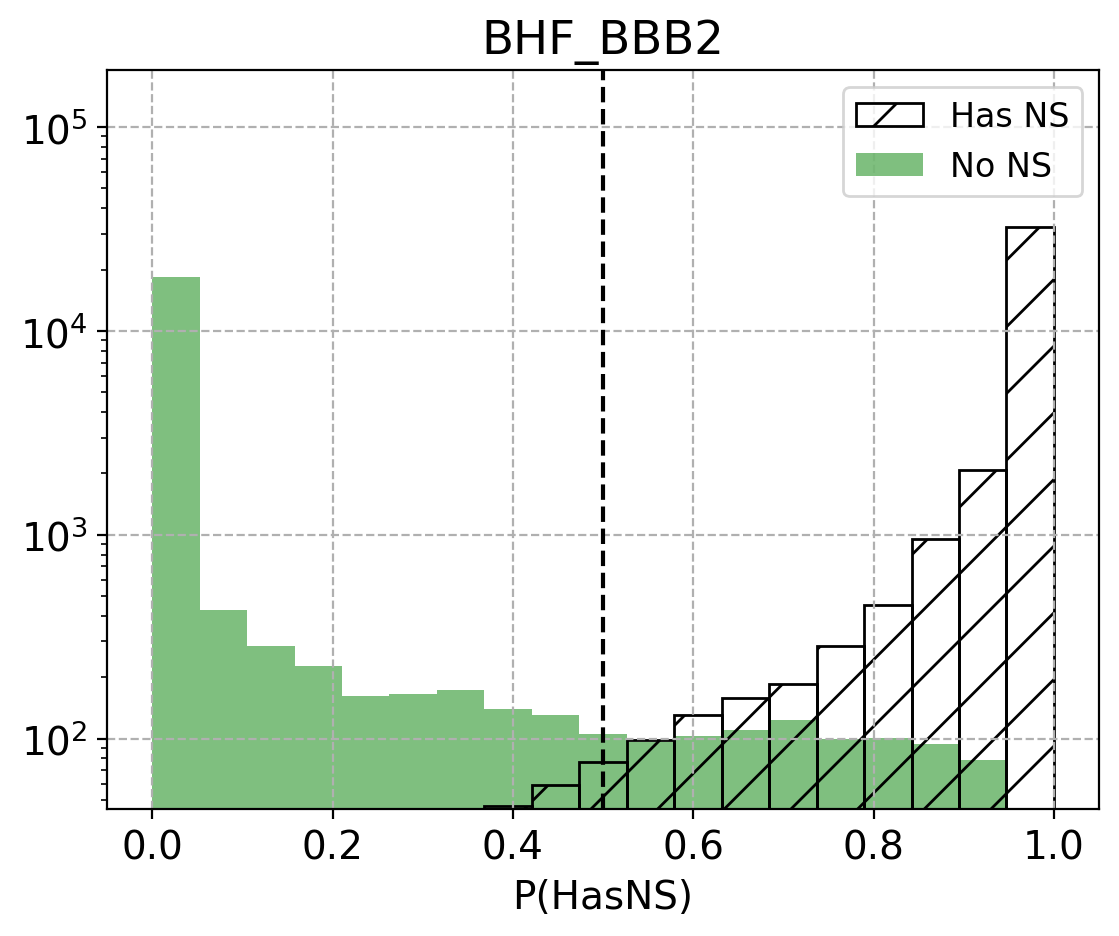
\includegraphics[width=0.45\textwidth]{/figs/BHF_BBB2_NShist}
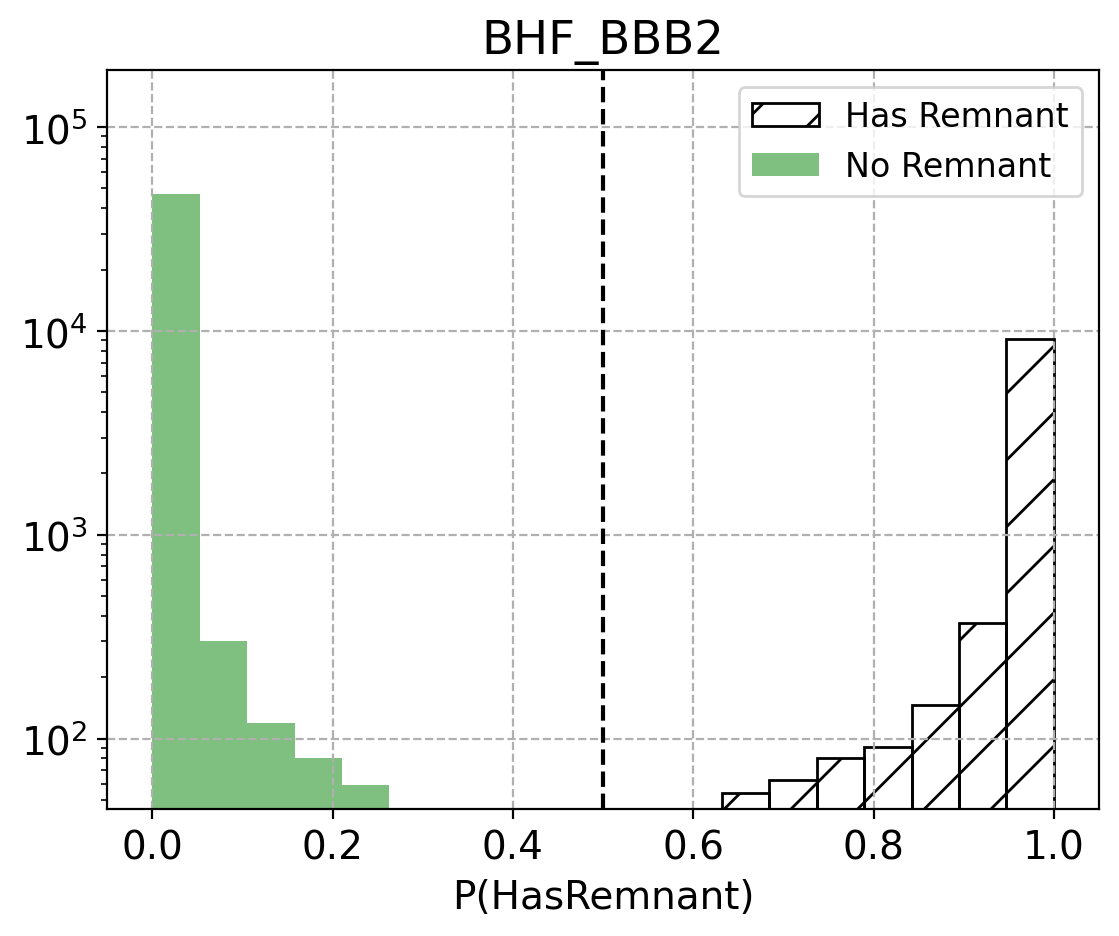
\includegraphics[width=0.45\textwidth]{/figs/BHF_BBB2_REMhist}
\caption{\label{fig:RF_hist_BHFBBB2} Histograms BHF BBB2}
\end{figure}

\begin{figure}
\centering
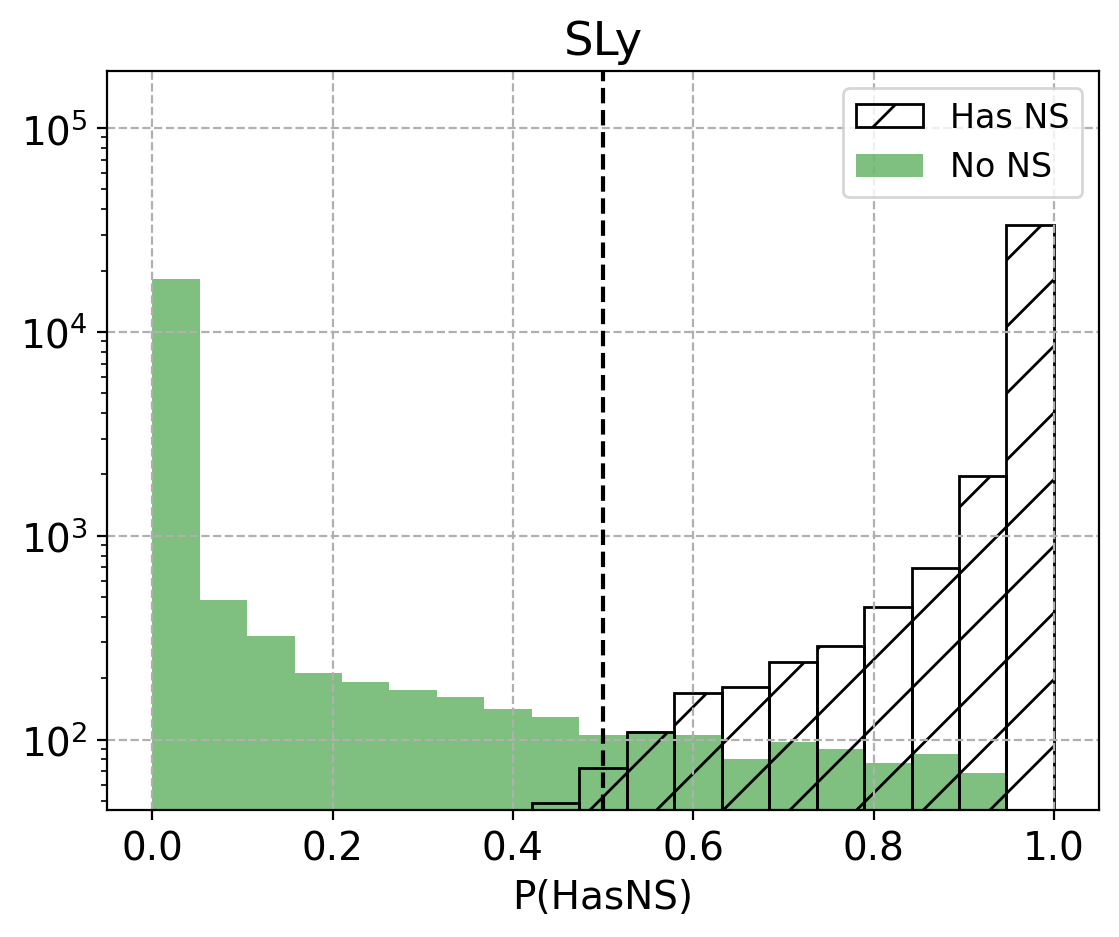
\includegraphics[width=0.45\textwidth]{/figs/SLy_NShist}
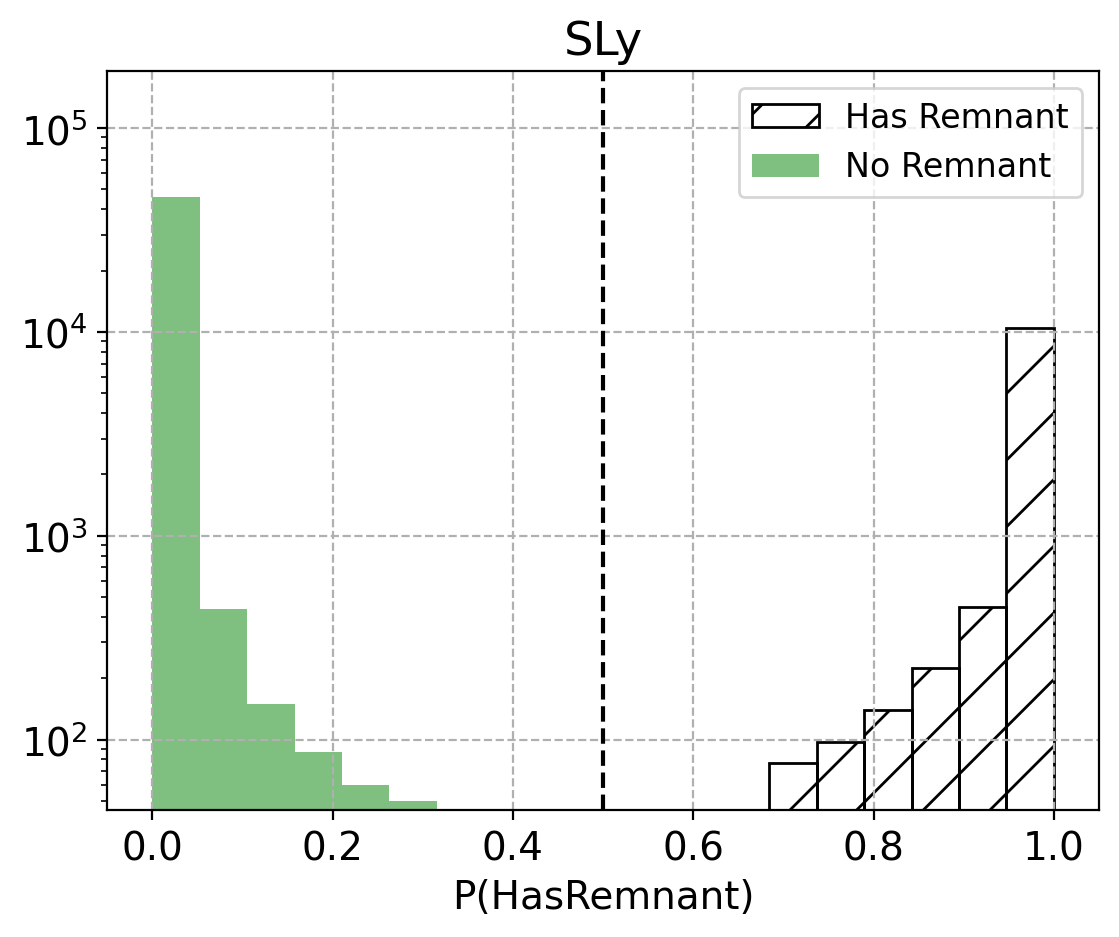
\includegraphics[width=0.45\textwidth]{/figs/SLy_REMhist}
\caption{\label{fig:RF_hist_SLY} Histograms SLy}
\end{figure}

\begin{figure}
\centering
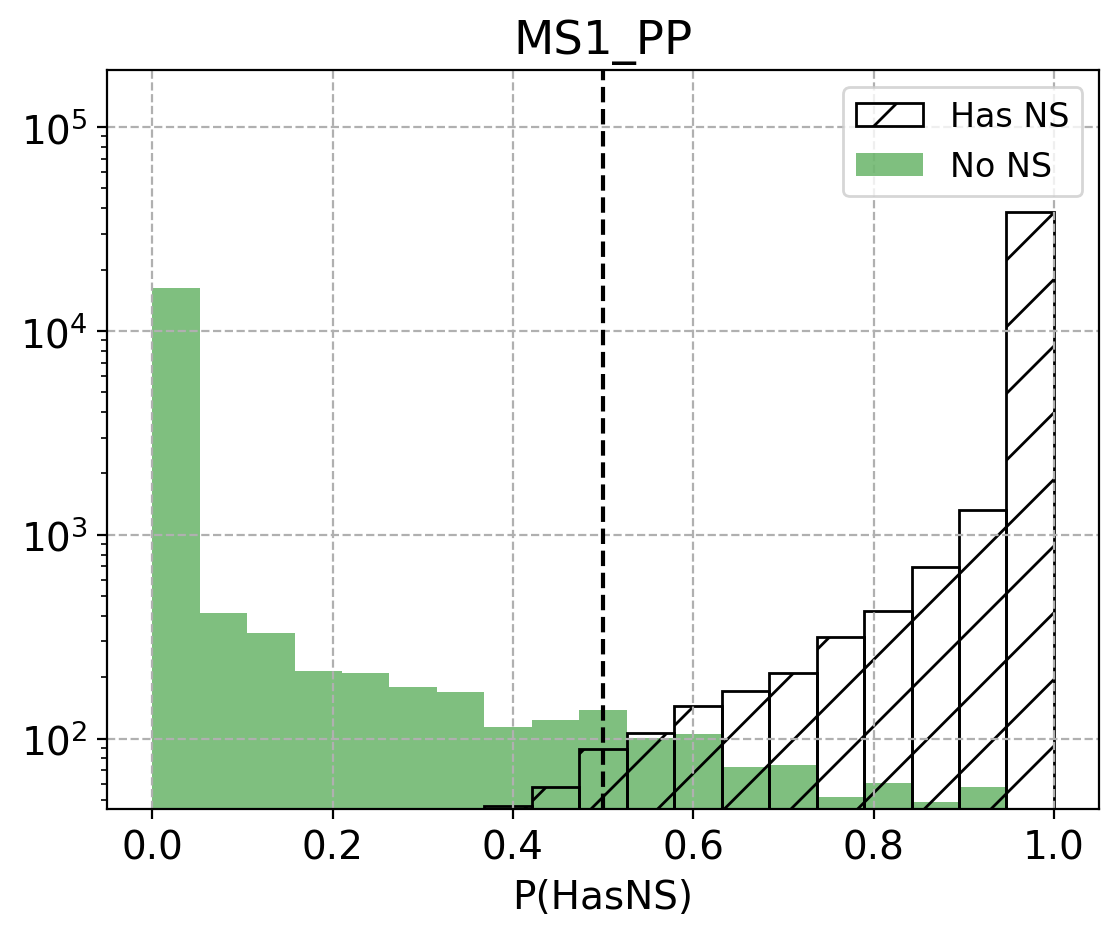
\includegraphics[width=0.45\textwidth]{/figs/MS1_PP_NShist}
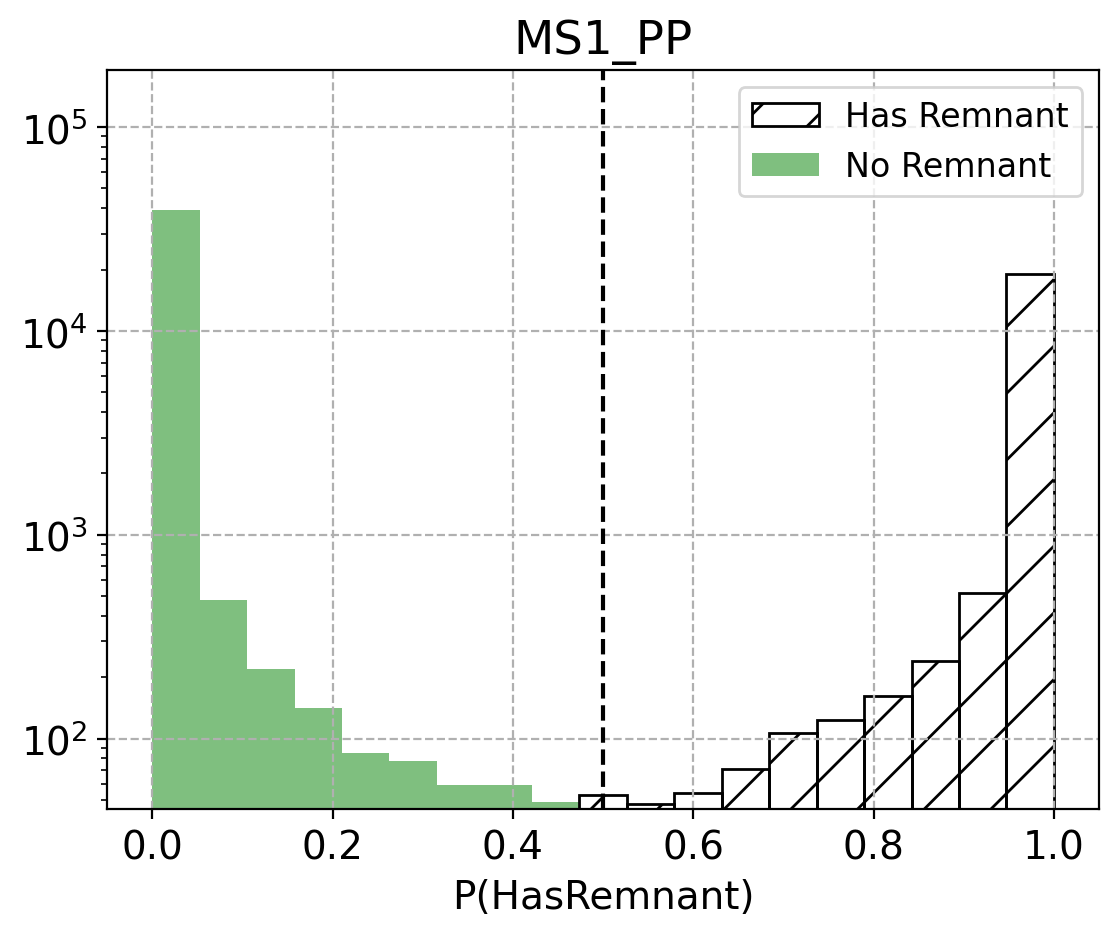
\includegraphics[width=0.45\textwidth]{/figs/MS1_PP_REMhist}
\caption{\label{fig:RF_hist_MS1PP} Histograms MS1 PP}
\end{figure}


 %plots and comments
%\input{GP_Results.tex}


%In order to decide which method gives a better performance in classifying this kind of events, we can apply them over testing data and finally do a comparison between both. A way to see how data is classified we can construct histograms where the number of events that are classified with a label (\texttt{HasNS/HasRemnant}) \texttt{True} or \texttt{False} will change with a given threshold of the probability. For an algorithm with perfect performance, all the events with label \texttt{True (False)} should be at \textit{p}(\texttt{label}) = 1 (\textit{p}(\texttt{label}) = 0).

%Another way to check the algorithm's performance is by building the so-called \textit{Receiver Operating Characteristic (ROC) Curve}. They show the variation of the true-positive rate (or efficiency) with the false-positive rate given a certain threshold for the probability. An algorithm with a proper performance will give a steeper ROC curve, or in other words, will have a higher eficiency with a lower false-positive rate.  


%In the ROC curves that we will present in the following subsections, we highlight three reference EoS in color, from which we show results in more detail. We select BHF\_BBB2 because is the model that give the lowest maximum mass, MS1\_PP as the model with the bigger maximum mass, and we also include SLy because is the most accepted EoS for NS modeling (reference), and is the one that was used in the injections that are our dataset.


%\subsection{Algorithm comparison}


%Here we talk about overall results and specifically from each algorithm in the
%subsections below.  \mmt{[MMT: Below I described how to check the performance of the algorithms. Maybe a table with all the scores/sensitivities/precisions from both %KNN and RF would be useful (already got it in a google doc)]}

%\mmt{To measure the performance of the classifiers we use some common statistical quantities.  The score is the number of correctly predicted events over the number %of total events (a perfect classifier has a score of 1).  It works best when there is an equal number of events for each label in the training set. It does not %consider the importance of misclassification, or that the training data can be biased towards one specific label.}

%\mmt{The mean score is computed by training the algorithm on the $90\%$ of the dataset and testing it on the remaining $10\%$, cycling the train/test combination over %the full dataset. To do that, we are going to use the training dataset, since it's the larger one.  In order to train and test the model and create the different %plots, we are going to use the training and testing files. }

%\mmt{Another useful quantity is the sensitivity. It is the ratio between the true positives and the sum of the true positives and false negatives.  It measures how %much the algorithm predicts \textit{true} (in our case it would be that the event has NS or has REM), when it is actually \textit{true}.Having a sensitivity equal to %1 would mean that our method predicts \textit{true} for every event. Therefore, a method with high sensitivity will barely miss true alarms. }

%\mmt{A quantity that measures how much you can trust a method when it predicts \textit{true} is the precision.  It is the ratio between the true positives and the %some of the true  and the false positives. A precision equal to 1 means that the method never predicts \textit{true} when it is actually \textit{false}. This means %that the method will never give false alarms. }

%\mmt{Finally, the F1 score $F1 = 2(\rm{precision \times sensitivity})/(\rm{precision+sensitivity})$ is a type of score that takes into consideration how precision and %sensitivity compensate each other. A perfect classifier would have a F1 score of 1.}

%To compare quantitatively the results from RF and KNN we compute the true positive and false positive rate for several threshold values, for both HasNS and HasREM, for the three selected EoS. These are tables \ref{tab:TPbhf}, \ref{tab:TPms1} and \ref{tab:TPsly}. For HasNS the two algorithms perform similarly, with almost the same TP for all threshold values and accross EoSs, although the false positive is smaller always in the RF. For HasREM we obtain that RF performs better than KNN in every case, with not only a smaller false positive rate, but a greater true positive rate.

%\begin{table}[]
%\centering
%\begin{tabular}{@{}c|cccc|cccc@{}}
%\toprule
%\multicolumn{1}{l|}{}          & \multicolumn{4}{c|}{Has NS}                       & \multicolumn{4}{c}{Has REM}                      \\ \midrule
%                               & \multicolumn{2}{c}{RF} & \multicolumn{2}{c|}{KNN} & \multicolumn{2}{c}{RF} & \multicolumn{2}{c}{KNN} \\
%\multicolumn{1}{l|}{Threshold} & TP         & FP        & TP          & FP         & TP         & FP        & TP         & FP         \\ \midrule
%0.1                            & 0.999      & 0.107     &   0.999          &  0.156          & 0.998      & 0.011     &    0.992        &  0.051          \\
%0.3                            & 0.998      & 0.068     &   0.996        &  0.117          & 0.993      & 0.005     &   0.974         &  0.017          \\
%0.5                            & 0.994      & 0.042     &   0.991          &  0.088           & 0.985      & 0.003     &   0.937         &  0.006          \\
%0.8                            & 0.967      & 0.014     &   0.966          & 0.043            & 0.957      & 0.001     &  0.845          &   0.001         \\ %\bottomrule
%\end{tabular}
%\caption{BHF\_BB2}
%\label{tab:TPbhf}
%\end{table}

